\documentclass[a4paper, 12pt]{article}
\usepackage[
  a4paper,
  top=3cm,
  bottom=3cm,
  left=2cm,
  right=2cm
]{geometry}
\setlength{\parskip}{1em}      % Espacio entre párrafos
\setlength{\parindent}{1.5em}    % Sangría al inicio de párrafo
\usepackage{forest}
\usepackage{xcolor}
\usepackage{mdframed}
\definecolor{shadecolor}{rgb}{0.1,0.1,0.1}
\usepackage[utf8]{inputenc}
\usepackage[T1]{fontenc}
\usepackage{textcomp}
\usepackage{amsmath, amssymb}
\usepackage{stmaryrd}
\usepackage{tikz}
\usetikzlibrary{shapes.geometric}
\usepackage{tikz-cd}
\usetikzlibrary{positioning}
\usepackage[cal=boondoxo, bb=ams]{mathalfa}
\usepackage{mlmodern}
\newtheorem{problem}{Problem}
\newtheorem{example}{Example}
\newtheorem{lemma}{Lemma}
\newtheorem{theorem}{Theorem}
\newtheorem{problem}{Problem}
\newtheorem{example}{Example} \newtheorem{definition}{Definition}
\newtheorem{lemma}{Lemma}
\newtheorem{theorem}{Theorem}
\usepackage[pdftex]{graphicx}
\newcommand\doubleplus{+\kern-1.3ex+\kern0.8ex}
\newcommand\mdoubleplus{\ensuremath{\mathbin{+\mkern-10mu+}}}
\DeclareGraphicsExtensions{.pdf,.jpeg,.png,.jpg}
\newmdenv[backgroundcolor=orange!25,
            leftline=false,
            rightline=false,
            bottomline=true,
            linewidth=2pt,
            linecolor=black]{myframe}
\newmdenv[backgroundcolor=blue!35,
            leftline=false,
            rightline=false,
            bottomline=true,
            linewidth=2pt,
            linecolor=black]{helpframe}


\begin{document}


\begin{titlepage}
   \begin{center}
       \vspace*{1cm}

       \Huge
       \textbf{Modelos y simulación - Prácticos}

       \vspace{0.5cm}
        FAMAF - UNC
            
       \vspace{1.5cm}
       \large
       \textbf{Severino Di Giovanni}
       \normalsize


       \vspace{5.0cm}
       \begin{figure}[h!]
       \centering
        
\includegraphics[width=0.5\textwidth]{../Images/UPA.jpg}
       \end{figure}

       \vfill
            
            
     
   \end{center}
\end{titlepage}


\shipout\null

 \begin{figure}[h!]
 \centering
  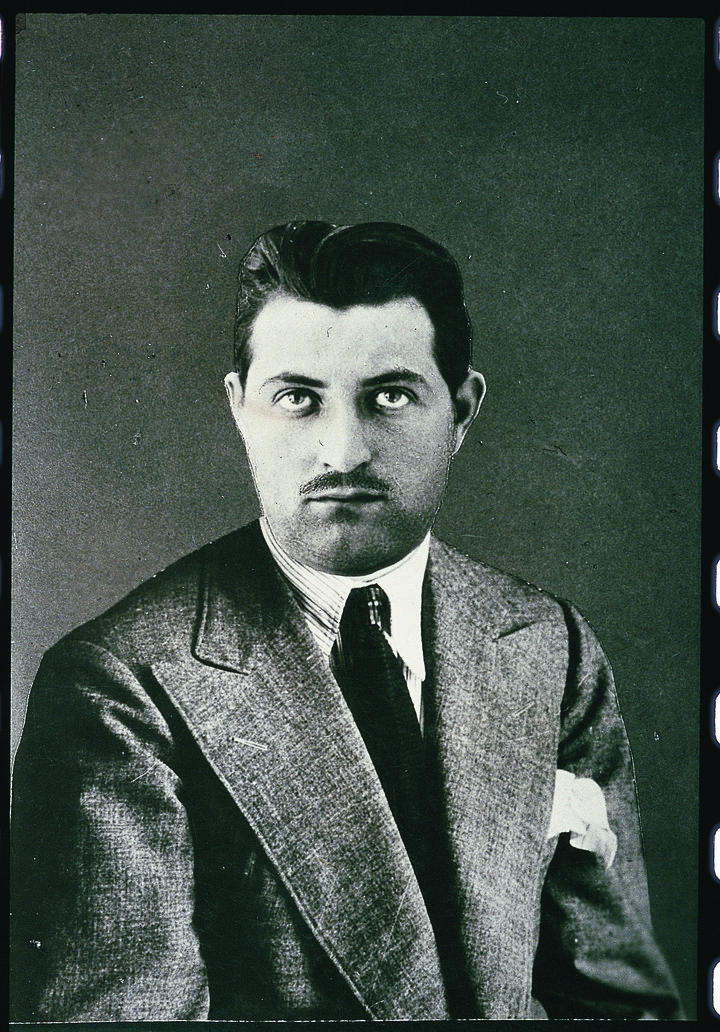
\includegraphics[width=0.5\textwidth]{../Images/SeverinoDiGiovanni.jpg}
 \caption{Severino Di Giovanni, el autor de este apunte. Un anarquista
   libertario, murió luchando por la libertad. Como él, otros miles han muerto
   para que nosotros gocemos de los derechos que tenemos. No te dejes engañar
   por los tristes pregoneros del egoísmo. Amá a tu prójimo y no olvides que si
   sus derechos se vulneran, los tuyos también. Ayudá a tu compañero de estudio,
 defendé tu universidad. }
 \end{figure}

\pagebreak
\tableofcontents
\newpage

\section{Teoría}

\subsection{Órdenes parciales y dominios}

\subsubsection{Órdenes discretos y llanos}

Al orden parcial dado por la relación $a \preceq b \iff a = b$ lo llamamos el
orden discreto. Ningún elemento es comparable con otro. Además, dados dos
conjuntos $X$ e $Y$, definimos el
siguiente orden sobre $X \to Y$:

\begin{equation*}
  f \leq g \iff x \in \mathcal{D}_f \Rightarrow x \in \mathcal{D}_g \land
  f(x) \leq_Y f(y)
\end{equation*}

Es fácil demostrar que este orden es parcial. 

~ 

Además, dado un conjunto $X$, definimos $X_\bot $ como la operación de
\textit{lifting} tal que 

\begin{equation*}
  X_\bot = \Big( X \cup \left\{ \bot  \right\}, \preceq  \Big)
\end{equation*}

con $\preceq$ idéntico al orden discreto, excepto que $\bot$ es menor (y por
ende comparable) a todos los elementos de $X$. Es fácil probar que $X_\bot $ es
un orden parcial. Al orden $\preceq$ dado por la operación de lifting se le
llama el \textbf{orden llano}. Si $X$ es un poset que posee un mínimo, usamos
$\bot $ para denotar dicho mínimo.

~ 

Si $X$ es un conjunto, definimos también 

\begin{equation*}
  X^\infty = \Big( X \cup \left\{ \infty \right\}, \preceq \Big)
\end{equation*}

donde $\preceq$ es el orden usual sobre $X$, excepto que $\infty$ es un máximo.


\begin{figure}[!h]
\centering
\begin{tikzpicture}
  % Nodo de abajo
  \node (bot) at (0,-2) {$\bot$};

  % Nodos de arriba (colocados manualmente con xshift)
  \node[above=1cm of bot, xshift=-3cm] (dots2) {$\ldots$};
  \node[above=1cm of bot, xshift=-2cm] (sigma1) {$-2$};
  \node[above=1cm of bot, xshift=-1cm] (sigma2) {$-1$};
  \node[above=1cm of bot, xshift=0cm] (dots1) {$0$};
  \node[above=1cm of bot, xshift=1cm] (Omega1) {$1$};
  \node[above=1cm of bot, xshift=2cm] (Omega2) {$2$};
  \node[above=1cm of bot, xshift=3cm] (dots2) {$\ldots$};

  % Conexiones
  \draw (bot) -- (sigma1);
  \draw (bot) -- (sigma2);
  \draw (bot) -- (dots1);
  \draw (bot) -- (Omega1);
  \draw (bot) -- (Omega2);
\end{tikzpicture}
\caption{Diagrama de Hasse de $\mathbb{Z}_\bot $}
\end{figure} 


\begin{figure}[!h]
\centering
\begin{tikzpicture}
  % Nodo de abajo
  \node (bot) at (0,-2) {$\bot = 0$};
  % Nodos de arriba (colocados manualmente con xshift)
  \node[above=1cm of bot] (one) {$1$};
  \node[above=1cm of one] (two) {$2$};
  \node[above=1cm of two] (ldots) {$\vdots$};
  \node[above=1cm of ldots] (inf) {$\infty$};

  % Conexiones
  \draw (bot) -- (one);
  \draw (one) -- (two);
  \draw (two) -- (ldots);
  \draw (ldots) -- (inf);
\end{tikzpicture}
\caption{Diagrama de Hasse de $\mathbb{N}$}
\end{figure} 

\subsubsection{Cadenas}

Una cadena $C$ de un poset $\mathcal{P}$ es una secuencia infinita $\left\{ p_i
\right\}_{i \in \mathbb{N}} $ tal que $p_0 \leq p_1 \leq \ldots$, donde $\leq$
es el orden asociado a $\mathcal{P}$. Si el conjunto $\left\{ p : p = p_i \text{
para algún } i \in \mathbb{N} \right\} $ es finito, decimos que la cadena es
no-interesante. Si es infinito, decimos que la cadena es interesante. Notemos
que el caso finito solo puede darse si, a partir de cierto $k \in \mathbb{N}$,
$p_k = p_{k+1} = p_{k+2} = \ldots$. Es fácil notar que los órdenes discretos y
llanos sólo tienen cadenas no-interesantes.

~

Si todas las cadenas de un orden parcial tienen supremo, decimos que dicho orden
es un \textbf{predominio}. En general, si $Y$ es un predominio, $X \to Y$ es un
predominio.



\small
\begin{quote}

\textbf{Prueba.} Asuma que $\left( Y, \leq_Y \right) $ es predominio. Entonces,
en particular, es un orden parcial. $\therefore $ Dado un conjunto $X$, tenemos
el orden parcial asociado a $X \to Y$ dado por 

\begin{equation*}
  f \leq g \iff \forall x \in X : x \in \mathcal{D}_f \Rightarrow x \in \mathcal{D}_g \land f(x)
  \leq_Y g(x)
\end{equation*}

Sea $f_1 \leq f_2 \leq \ldots$ una cadena arbitraria de $X \to Y$. Si dicha
cadena es no-interesante, necesariamente tiene supremo, así que estudiemos el
caso en que la cadena es interesante. Dado $x_0 \in \mathcal{D}_{f_1}$ arbitrario, la cadena
$f_1 \leq f_2 \leq \ldots$ induce una cadena en $Y$ dada por 

\begin{equation*}
  f_1(x_0) \leq f_2(x_0) \leq \ldots
\end{equation*}

Por hipótesis, dicha cadena tiene un supremo $\bigsqcup_{i \in \mathbb{N}}
f_i(x_0)$. Si definimos 

$$\mathcal{F}(x_0) = \bigsqcup_{i \in \mathbb{N}} f_i(x_0)$$

tenemos que $\mathcal{F} \in (X \to Y)$, que $x_0 \in \mathcal{D}_{f_i}
\Rightarrow x_0\in \mathcal{D}_{\mathcal{F}}$, y que para todo $i$ se cumple
$f_i(x_0) \leq \mathcal{F}(x_0)$. $\therefore $ $\mathcal{F}$ es cota superior
de $f_1 \leq f_2 \leq \ldots$ Que es supremo se sigue fácilmente de que 
$\bigsqcup_{i \in \mathbb{N}} f_i(x_0)$ es supremo de $f_1(x_0) \leq f_2(x_0)
\leq \ldots$


\end{quote}
\normalsize

Un predominio que tiene un elemento mínimo se denomina \textbf{dominio}. Aquí
otra vez se cumple que si $D$ es dominio, $X \to D$ es dominio.

\small
\begin{quote}

\textbf{Prueba.} Asuma que $D$ es dominio. Entonces es predominio y por lo tanto
$X \to D$ es predominio. Sea $\psi \in X \to D$ definida como la función
constante $\psi = \bot_D$. Entonces es claro que $\psi \leq f$ para toda $f \in
X \to D$. Luego $\psi$ es mínimo de $X \to D$.


\end{quote}
\normalsize

\subsection{Morfismos y funciones continuas}

Sean $X, Y$ posets. Si $f \in X \to Y$ preserva el orden parcial, se dice
monótona. Si $f$ preserva además el supremo de cadenas, se dice continua. Si
además preserva el mínimo, se dice estricta.

Debería ser claro que si $x_1 \leq x_2 \leq \ldots$ es una cadena en $X$ y $f
\in X \to Y$ es monótona, entonces $f(x_1) \leq f(x_2) \leq \ldots$ es una
cadena en $Y$. Cabe también destacar que si $f$ es monótona, preserva el supremo
de cadenas no-interesantes. Por lo tanto, podríamos definir la noción de
continuidad como la preservación de supremos en cadenas interesantes.


\small
\begin{quote}

  \textbf{Ejemplo.} Considere $f \in \mathbb{N}^\infty \to \left\{ \top, \bot
  \right\} $. Asuma que $f(n) = \bot $ para todo $n \in \mathbb{N}$ y que
  $f(\infty) = \top$. Claramente, $f$ es monótona, pero no preserva el supremo
  de $1 \leq 2 \leq 3\ldots$ Aplicar $f$ dicha cadena da $\bot  \leq \bot  \leq
  \ldots$ con supremo $\bot \neq f(\infty)$.

\end{quote}
\normalsize

Aunque la monotonía no implica continuidad, una función monótona en $X \to Y$ nos da una cota
superior para el supremo de las cadenas de $Y$.

\begin{theorem}
  Si $P, Q$ son predominios y $f \in P \to Q$ es monótona, 

  \begin{equation*}
    \bigsqcup_{i \in \mathbb{N}} f(p_i) \leq f \left( \bigsqcup_{i \in
    \mathbb{N}} p_i \right) 
  \end{equation*}
\end{theorem}



\small
\begin{quote}

\textbf{Prueba.} Sea $f : P \mapsto Q$ monótona y $p_0 \leq_P p_1 \leq_P \ldots$
una cadena interesante de $P$.  

Para todo $j$ se cumple $p_j \leq \bigsqcup_{i \in \mathbb{N}} p_i$. Como $f$ es
monótona, $f(p_j) \leq f\left( \bigsqcup_{i \in \mathbb{N}} p_i \right) $. 

$\therefore $ $f\left( \bigsqcup_{i \in \mathbb{N}} p_i \right) $ es cota
superior de $\left\{ f(p_i) \right\}_{i \in \mathbb{N}} $.

Como $Q$ es predominio, la cadena $\left\{ f(p_i) \right\}_{i \in \mathbb{}} $
tiene supremo. Como por def. dicho supremo es la menor cota superior,

\begin{equation*}
  \bigsqcup_{i \in \mathbb{N}} f(p_i) \leq f \left( \bigsqcup_{i \in \mathbb{N}}
  p_i\right) \qquad \blacksquare
\end{equation*}



\end{quote}
\normalsize

Es fácil demostrar que si $f$ es monótona entonces es continua. De este hecho y
del teorema anterior se sigue que $f$ es continua si y solo si 

\begin{equation*}
  f\left( \bigsqcup_{i \in \mathbb{N}} p_i \right) = \bigsqcup_{i \in
  \mathbb{N}} f(p_i)
\end{equation*}


\subsection{Extensión de funciones para lenguajes con fallas}

Un estado abortivo, o estado con falla, es un par $\left<\textbf{abort}, \sigma
\right>$, donde $\textbf{abort}$ es una nueva palabra del lenguaje y $\sigma$
es un estado. Definimos

\begin{equation*}
  \hat{ \Sigma }  := \Sigma \cup \left\{ \left<\textbf{abort}, \sigma \mid
  \sigma \in \Sigma\right> \right\} = \Sigma \cup  \left\{ \textbf{abort}
  \right\}  \times \Sigma
\end{equation*}

y

\begin{equation*}
  \llbracket \textbf{fail} \rrbracket ~ \sigma := \left<\textbf{abort}, \sigma \right>
\end{equation*}

Ahora damos la siguiente extensión. Si $f \in \Sigma \mapsto \widetilde{
\Sigma_\bot  } $, definimos $f_* :
\widetilde{ \Sigma_\bot  } \mapsto \widetilde{ \Sigma_\bot  }$ como

\begin{equation*}
  f_*(\omega) = \begin{cases}
    \bot  & \omega = \bot  \\ 
    f ~ \omega & \omega \in \Sigma \\ 
    \left<\textbf{abort}, \sigma \right> & \omega = \left<\textbf{abort}, \sigma \right>
  \end{cases}
\end{equation*}

Entonces se tiene

\begin{equation*}
  \llbracket c_0;c_1 \rrbracket ~ \sigma = \left( \llbracket c_1 \rrbracket
  \right)_{*} ~ \left( \llbracket c_0 \rrbracket ~ \sigma\right) 
\end{equation*}

Análogamente,

\begin{align*}
  \llbracket \textbf{while } b \textbf{ do } c \rrbracket &= \bigsqcup_{i \in
  \mathbb{N}} F^i ~ \bot  \\ 
    \text{ where } F ~ f ~ \sigma &= \begin{cases}
    f_{*}(\llbracket c \rrbracket ~ \sigma) & \llbracket b \rrbracket \\ 
    \sigma & \text{otherwise}
  \end{cases}
\end{align*}


Si $f \in \Sigma \mapsto \Sigma$, definimos $f_\dagger \in \widetilde{
\Sigma_\bot  } \mapsto \widetilde{ \Sigma_\bot  } $ como:

\begin{equation*}
  f_\dagger ~ \omega = \begin{cases}
    \bot  & \omega = \bot  \\ 
    f ~ \sigma & \sigma \in \Sigma \\ 
    \left<\textbf{abort}, f ~ \sigma \right> & \omega = \left<\textbf{abort}, \sigma \right>
  \end{cases}
\end{equation*}

Entonces

\begin{align*}
  &\llbracket \textbf{newvar } v := e \textbf{ in } c\rrbracket ~ \sigma \\ 
  &\qquad = \left( \lambda \sigma' \in \Sigma . [\sigma' \mid v : \sigma ~ v]
  \right)_{\dagger} \left( \llbracket c \rrbracket [\sigma \mid v : \llbracket e
  \rrbracket] ~ \sigma \right) 
\end{align*}

\pagebreak
\subsection{Output}


Una vez incorporado el output a nuestro lenguaje, hay tres maneras en que un
programa se puede comportar:

\begin{itemize}
  \item El programa produce una secuencia finita y luego se ejecuta indefinidamente sin generar más salida.
  \item El programa produce una secuencia finita y luego termina normalmente o de forma abortiva.
  \item El programa produce una secuencia infinita.
\end{itemize}

Definimos $\Omega$ como el dominio de salida y determinamos que $\Omega$ está ordenado como sigue:

\begin{equation*}
  \omega \sqsubseteq \psi \iff \omega \text{ es subsecuencia inicial de } \psi
\end{equation*}

Ahora consideremos una cadena $\left\{ \omega_i \right\}_{i \in \mathbb{N}}$. Si $\left\{\omega_i\right\}_{i \in \mathbb{N}}$ no es interesante, su supremo será una secuencia finita de enteros o una secuencia finita con enteros y un último elemento que es un estado. Si $\left\{\omega_i\right\}_{i \in \mathbb{N}}$ es interesante, entonces cada $\omega_i$ es la "instantánea" de una computación infinita en los tiempos $i = 1, 2, \ldots$. Por ejemplo, en la computación de los dígitos de $\pi$, tendríamos:

\begin{equation*}
  \left< \right> \sqsubseteq \left< 3 \right> \left<3, 1 \right> \left<3,1,4 \right> \sqsubseteq \left<3, 1, 4, 1 \right> \sqsubseteq  \left<3, 1, 4, 1, 5 \right> \sqsubseteq  \left<3, 1, 4, 1, 5, 9 \right> \sqsubseteq  \ldots
\end{equation*}

Entonces el límite de la cadena es el elemento del dominio que describe la
salida total de la computación. No es difícil notar que $\Omega$ es un dominio.

\small
\begin{quote}

\textbf{Prueba.} Los casos finitos son triviales. Sea $\{ \omega_i \}_{i \in \mathbb{N}}$ una secuencia infinita con $\omega_i \in \Omega$.

Dado que $\omega_i \sqsubseteq \omega_{i+1}$ y estas secuencias son distintas y finitas, $\omega_{i+1}$ tiene más elementos que $\omega_i$. Además, si $\omega_i$ tiene un elemento $j$-ésimo, entonces $\omega_{i+1}$ también lo tiene, y estos coinciden. Por lo tanto, cualquier cota superior de la cadena es una secuencia infinita.

Además, si $\mu$ es una cota superior de la cadena, el $i$-ésimo elemento de $\mu$ debe ser idéntico al $i$-ésimo elemento de todas las secuencias de la cadena cuya longitud sea al menos $i$. En otras palabras, para todo $i \in \mathbb{N}$, el $i$-ésimo elemento de $\mu$ está determinado de manera única. $\therefore$ $\mu$ es único.

Dado que cualquier cota superior de la cadena está determinada de manera única, la cadena tiene una sola cota superior, y por lo tanto debe ser la menor cota superior.

$\therefore$ $\Omega$ es un predominio.

Es trivial observar que la secuencia vacía $\left< \right> \in \Omega$, que es la salida de un programa que se ejecuta indefinidamente sin realizar ninguna operación de escritura, es el mínimo.

$\therefore$ $\Omega$ es un dominio.

\end{quote}
\normalsize

\pagebreak 
\subsection{Extensión de outputs}

Sea $f : \Sigma \mapsto \Omega$ una función de estados en outputs. La extensión
de $f$ definida como $f_* : \Omega \mapsto \Omega$ se define como

\begin{equation*}
  f_* ~ \omega = \begin{cases}
    \left<n_0, \ldots, n_{k-1} \right> \doubleplus f ~ \sigma & \omega =
    \left<n_0, \ldots, n_{k-1}, \sigma \right> \\ 
    \omega & c.c.
  \end{cases}
\end{equation*}

Es decir que $f_*$ es inefectiva (es la función identidad) para todo $\omega \in
\Omega$ que no tiene un estado final $\sigma$. Esto incluye los outputs infinitos, los
outputs finitos sin estado final, y los outputs que terminan en
$\left<\textbf{abort}, \sigma \right>$.

Esta función nos permite definir la concatenación de comandos:

\begin{equation*}
  \llbracket c_0;c_1 \rrbracket \sigma = \left( \llbracket c_1 \rrbracket
  \right)_* \left( \llbracket c_0 \rrbracket \sigma \right) 
\end{equation*}

\textbf{Ejemplo.} Si $\llbracket c_0 \rrbracket \sigma$ termine en $\left<1, 2,
\sigma'\right>$ y $\llbracket c_1 \rrbracket\sigma'$ termina en $\left<3, 4
, \gamma\right>$, $\llbracket c_0;c_1 \rrbracket\sigma = \left<1, 2, 3, 4
, \gamma\right>$.

También nos permite definir el \textbf{while} de manera que el estado final es
inyectado a una secuencia, con $\llbracket \textbf{while } b \textbf{ do } c
\rrbracket\sigma = \bigsqcup_{i \in \mathbb{N}} F^i ~ \bot $ y

\begin{equation*}
  F ~ f ~ \sigma = \begin{cases}
    \left<\sigma \right> & \neg\llbracket b \rrbracket\sigma \\ 
    f_* (\llbracket c \rrbracket \sigma) & c.c.
  \end{cases}
\end{equation*}

Notemos que al usar $f_*$, el output de cada iteración del \textbf{while} será
concatenado al output de la iteración anterior.

\subsubsection{Transformación de estados finales}

Si $f \in \Sigma \to  \Sigma$, $f_\dagger : \Omega\to \Omega$ se define como 

\begin{equation*}
  f_\dagger ~ \omega = \begin{cases}
    \left<n_0, \ldots, n_{k-1}, \left<\textbf{abort}, f ~ \sigma \right> \right>
    & \omega = \left<n_0,\ldots, n_{k-1}, \left<\textbf{abort}, \sigma \right>
    \right> \\ 
    \left<n_0, \ldots, n_{k-1}, f ~ \sigma \right> & \omega = \left< n_0,
    \ldots, n_{k-1}, \sigma\right> \\ 
    \omega & c.c.
  \end{cases}
\end{equation*}

Es decir, $f_\dagger ~ \omega$ aplica $f$ al estado final de $\omega$, incluso
si dicho estado final es el estado en que se produjo una falla. Esto nos permite
definir 

\begin{equation*}
  \llbracket \textbf{newvar } v := e \textbf{ in } c\rrbracket\sigma = \mathcal{R}_\dagger \left( \llbracket c \rrbracket[\sigma \mid v :
  \llbracket e \rrbracket \sigma] \right) 
\end{equation*}

donde $\mathcal{R}$ es la restauración:

\begin{equation*}
  \mathcal{R} := \lambda \sigma' \in \Sigma . \llbracket \sigma' \mid v : \sigma
  ~ v\rrbracket
\end{equation*}

\subsection{Abstrayendo $\Omega$}

Ahora nos proponemos expresar la extensión $f_*$ de $f$ en función de cuatro
inyeciones disjuntas. Dichas inyecciones son:

\begin{align*}
  &(1) ~ ~ ~ \iota_\bot \in \left\{ \left< \right> \right\} \to \Omega \qquad \text{ definida como
  } \qquad \iota_\bot () = \left< \right> = \bot_\Omega\\
  &(2) ~ ~  ~\iota_{\text{term}} \in \Sigma \to \Omega \qquad \text{ definida como
  } \qquad \iota_{\text{term}}(\sigma) = \left<\sigma \right>\\
  &(3) ~ ~ ~ \iota_{\text{abort}} \in \Sigma \to \Omega \qquad \text{ definida como
  } \qquad \iota_{\text{abort}} (\sigma) = \left<\left<\textbf{abort}, \sigma \right> \right>\\
  &(4)~ ~ ~ \iota_{\text{out}} \in \mathbb{Z} \times \Omega \to \Omega \qquad \text{ definida como
  } \qquad \iota_{\text{out}}(n, \omega) = \left<n \right> \doubleplus \omega
\end{align*}

\begin{align*}
  f_* ~ \bot &= \bot  \\ 
  f_*(\iota_\text{term} ~ \sigma) &= f ~ \sigma \\ 
  f_*(\iota_{\text{abort}} \sigma) &= \iota_{\text{abort}} ~ \sigma \\ 
  f_*(\iota_{\text{out}}(n, \omega)) &= \iota_{\text{out}}(n, f_* \omega)
\end{align*}

Un primer punto interesante es que ahora la definición de $f_*$ para el caso de un
output $\left<n_0, \ldots, n_{k-1}, \ldots\right>$ es recursiva. También es
importante notar que las funciones $\iota$ son inyectivas y tienen rangos
disjuntos, y que cualquier $\omega \in \Omega$ finito puede formarse a través de
sucesivas aplicaciones de estas funciones. Es decir, podemos pensar que estas
funciones son constructores de una sintaxis abstracta cuyas frases son las
secuencias finitas de $\Omega$.

Análogamente, se puede definir 

\begin{align*}
  f_\dagger\left< \right> &= \left< \right> \\ 
  f_\dagger \left<\sigma \right> &= \left<f ~ \sigma \right> \\ 
  f_\dagger \left<\left<\textbf{abort}, \sigma \right> \right> &=
  \left<\left<\textbf{abort}, f ~\sigma \right> \right> \\ 
  f_\dagger \left( \left<n \right> \doubleplus \omega \right) &= \left<n \right>
  \doubleplus f_\dagger ~ \omega
\end{align*}
\pagebreak
\subsubsection{Isomorfismos sobre $\Omega$}

El dominio $\Omega$ tiene el siguiente orden:

~
\begin{figure}[!h]
\centering
\begin{tikzpicture}
  % Nodo de abajo
  \node (bot) at (0,-2) {$\bot = \left< \right>$};

  % Nodos de arriba (colocados manualmente con xshift)
  \node[above=1cm of bot, xshift=-3cm] (sigma1) {$\left<\sigma_1 \right>$};
  \node[above=1cm of bot, xshift=-2cm] (sigma2) {$\left<\sigma_2 \right>$};
  \node[above=1cm of bot, xshift=-1cm] (dots1) {$\ldots$};
  \node[diamond, draw, above=1cm of bot, xshift=0cm] (Omega1) {$\Omega_1$};
  \node[diamond, draw,above=1cm of bot, xshift=1.5cm] (Omega2) {$\Omega_2$};
  \node[above=1cm of bot, xshift=2.5cm] (dots2) {$\ldots$};

  % Conexiones
  \draw (bot) -- (sigma1);
  \draw (bot) -- (sigma2);
  \draw (bot) -- (dots1);
  \draw (bot) -- (Omega1);
  \draw (bot) -- (Omega2);
  \draw (bot) -- (dots2);
\end{tikzpicture}
\end{figure} 
 


donde $\left<\sigma_i \right>$ son secuencias con un único estado o un único par
$\left<\textbf{abort}, \sigma \right>$, y el diamante con $\Omega_k$ es el conjunto de
secuencias que empiezan con el entero $k$.

~

\textbf{Autosimilitud de $\Omega$}. Considere lo siguiente: para cada $\omega \in \Omega_k$, existe una única
secuencia $\omega'\in \Omega$ tal que $\omega = k \doubleplus \omega'$. Es
decir, existe una correspondencia uno a uno entre todos elementos de $\Omega_k$ y
todos los elementos de $\Omega$, y es fácil ver que dicha correspondencia es
invertible. $\therefore $ $\Omega_k$ es isomórfico a $\Omega$.

\begin{quote}
$(\star)$ Informalmente, podemos pensar que ciertos elementos de $\Omega$ se parecen a
$\Omega$, o que $\Omega$ tiene subconjuntos que difieren muy poco del mismo
$\Omega$.
\end{quote}
~ 

\textbf{Naturaleza recursiva de $\Omega$}. Considere $\mathbb{Z} \times \Omega$ con $\mathbb{Z}$ bajo el orden discreto.
Claramente, para cada $k \in \mathbb{Z}$, existe $(k, \omega)$ para cada $\omega
\in \Omega$. Es decir, se asocia una "copia" de $\Omega$ a cada entero. El orden
punto a punto resulta 

\begin{equation*}
  \left<n, \omega \right> \sqsubseteq \left<n', \omega' \right> 
\iff n = n' \text{ y } \omega
  \sqsubseteq_\Omega \omega'
\end{equation*}

Es decir, cada "copia" tiene el mismo order que en $\Omega$, y los miembros de
copias diferentes son incomparables. Por lo tanto, cada $\left<n,
\omega\right>$ se corresponde con un único $\omega' \in \Omega_k$, y tenemos que 

\begin{equation*}
  \bigcup_{k \in \mathbb{Z}} \Omega_k \simeq \mathbb{Z} \times \Omega
\end{equation*}

Por lo tanto, combinando que la unión de los $\Omega_k$ es isomórfica a $\mathbb{Z} \times
\Omega$ con el orden de $\Omega$ dado en el primer diagrama, tenemos

\begin{figure}
\centering
\begin{tikzpicture}
  % Nodo de abajo
  \node (bot) at (0,-1) {$\bot$};

  % Nodos de arriba (colocados manualmente con xshift)
  \node[box, draw, above=1cm of bot, xshift=-2cm] (Sigma) {$\hat{\Sigma}$};
  \node[box, draw, above=1cm of bot, xshift=2cm] (ZOm) {$\mathbb{Z} \times \Omega$};
  % Conexiones
  \draw (bot) -- (Sigma);
  \draw (bot) -- (ZOm);
\end{tikzpicture}
\end{figure} 

~

~ 

~ 


~ 

En conclusión,

\begin{equation*}
  \Omega \simeq \left( \hat{\Sigma} + \mathbb{Z} \times \Omega \right) 
\end{equation*}

Por lo tanto, existen funciones continuas $\varphi, \psi$

\begin{equation*}
  \Omega 
\underset{\psi}{\overset{\phi}{\rightleftarrows}} 
\left( \hat{\Sigma} + \mathbb{Z} \times \Omega \right)_{\perp}
\end{equation*}

tales que $\varphi \circ \psi, \psi \circ \varphi$ son funciones identidad.

~

\begin{helpframe}
  Esto revela la naturaleza recursiva de $\Omega$ porque nos dice que todo
  elemento de $\Omega$ es o bien una secuencia con un único estado (tal vez
  abortivo), o bien $\bot$, o bien (caso recursivo) un entero pareado con otro
  elemento de $\Omega$.
\end{helpframe}

~

En particular, parear cada elemento de $\hat{\Sigma}$ con $0$ y cada elemento de
$\mathbb{Z} \times \Omega$ con $1$ no cambia ninguno de los resultados
anteriores. Por lo tanto, podemos descomponer $\Omega$ del siguiente modo:

\[
\begin{tikzcd}[row sep=large, column sep=huge]
\Sigma \arrow[dr, "\iota_{\text{norm}}"'] & \\
\Sigma \arrow[r, "\iota_{\text{abnorm}}"'] & \hat{\Sigma} \arrow[r, "\iota_0"] &
\hat{\Sigma}+ \mathbb{Z} \times \Omega \arrow[r, "\iota_{\uparrow}"] & (\hat{\Sigma} + \mathbb{Z} \times \Omega)_{\perp} \arrow[r, "\psi"] & \Omega \\
& & \mathbb{Z} \times \Omega \arrow[u, "\iota_1"']
\end{tikzcd}
\]
Acá, $\iota_{\text{norm}}, \iota_{\text{abnorm}}$ inyectan estados en
$\hat{\Sigma}$, mapeando $\sigma \mapsto \sigma$ y $\sigma \mapsto
\left<\textbf{abort}, \sigma \right>$, respectivamente. Las funciones $\iota_0,
\iota_1$ son la unión disjunta y $\iota_\uparrow$ es simplemente el lifting.
Tenemos entonces:

\begin{align*}
  \iota_{\text{term}} &= \psi \circ l_{\uparrow} \circ \iota_0 \circ
  \iota_\text{norm} \in \Sigma \to \Omega \\ 
  \iota_{\text{abort}} &= \psi \circ l_{\uparrow} \circ \iota_0 \circ
  \iota_\text{abnorm} \in \Sigma \to \Omega\\
  \iota_{\text{out}} &= \psi \circ l_{\uparrow} \circ \iota_1 \in (\mathbb{Z}
  \times \Omega) \to \Omega
\end{align*}

Dar las inyecciones en términos de la relación entre estos conjuntos, y no en
términos de la semántica de los mismos, nos permite librarnos del requisito de
que el dominio $\Omega$ sea una secuencia de enteros y estados. Cualquier grupo
de conjuntos donde las $\iota$ sean inyecciones con rangos disjuntos satisface
las propiedades requeridas.

\subsection{Input y nueva extensión de $\Omega$}

Si agregamos $\text{<comm>} ::= ?\text{<var>}$ al lenguaje, que hace que una
variable tome un valor dado por input, debemos extender la semántica todavía
más. Recordemos que, sin input, con $\Omega \simeq (\hat{\Sigma} + \mathbb{Z}
\times \Omega)_\bot $, habían cuatro posibilidades para un programa
$\mathcal{P}$:

\begin{itemize}
  \item $\mathcal{P}$ no se detiene y $\omega = \bot $.
  \item $\mathcal{P}$ termina en $\sigma$, y $\omega = \iota_{\text{term}} ~
    \sigma$. 
  \item $\mathcal{P}$ aborta en $\sigma$ y $\omega = \iota_{\text{abort}} ~
    \sigma$. 
  \item $\mathcal{P}$ escribe un $k \in \mathbb{Z}$ y luego se comporta según
    $\omega'$, es decir $\omega = \iota_{\text{out}}(k, \omega')$.
\end{itemize}

Para describir input, introducimos una posibilidad nueva, donde el input es
representado por una función $g \in \mathbb{Z} \to \Omega$:

\begin{itemize}
  \item $\mathcal{P}$ lee un entero $k$ y su comportamiento es determinado por
    $g ~ k$. En este caso decimos $\omega = \iota_{\text{in}} ~ g$ con $g \in
    \mathbb{Z} \to \Omega$.
\end{itemize}

Habiendo añadido esta posibilidad, tenemos que tomar $\Omega$ como una solución
de 

\begin{equation*}
  \Omega \simeq \left( \hat{\Sigma} + \left( \mathbb{Z} \times \Omega \right) +
  \left( \mathbb{Z} \mapsto \Omega \right) \right)_\bot 
\end{equation*}

Las ocurrencias de $\Omega$ que están en $\mathbb{Z} \to \Omega$ son llamadas
\textit{resumptions}, porque refieren comportamientos que se dan cuando el
proceso se resume después de input o output. Se define 

\begin{equation*}
  \iota_{\text{in}} = \psi \circ l_{\uparrow} \circ \iota_2 \in \left(
  \mathbb{Z} \to \Omega \right) \to \Omega
\end{equation*}


\subsection{El orden de $\Omega$}

Recordemos que, con input, output y fallas, determinamos que

  
\begin{equation*}
  \Omega \simeq \left( \hat{\Sigma} + \left( \mathbb{Z} \times \Omega \right) +
  \left( \mathbb{Z} \mapsto \Omega \right) \right)_\bot, \qquad 
  \Omega 
\underset{\psi}{\overset{\phi}{\rightleftarrows}} 
\left( \hat{\Sigma} + \mathbb{Z} \times \Omega \times \mathbb{Z} \to \Omega \right)_{\perp}
\end{equation*}

Una de las ventajas de pensar $\Omega$ como isomórfico al término derecho es que
el mismo hace evidente algunos puntos esenciales:

\begin{itemize}
  \item Todo elemento de $\Omega$ se corresponde con o bien un elemento de $\hat{\Sigma}$, o bien
    se define recursivamente como un entero asociado a un elemento de $\Omega$, 
    o bien es una función en $\mathbb{Z} \to \Omega$. 
  \item Todo $\omega \in \Omega$ finito es construido via
    inyecciones $\iota$, lifting, y $\psi$ a partir de los conjuntos
    $\hat{\Sigma}, \mathbb{Z} \times \Omega$ y $\mathbb{Z} \to \Omega$.
\end{itemize}

Notemos además que $\hat{\Sigma}$ y $\hat{\Omega}$ son predominios (carecen de
mínimo), mientras que $\mathbb{Z} \to \Omega$ es un dominio con mínimo $\lambda
n . \left< \right>$. El orden de $(\hat{\Sigma} + \mathbb{Z} \times \Omega +
\mathbb{Z} \to \Omega)$ es:



\tikzset{
  box/.style={draw, rectangle, rounded corners, align=center, minimum height=2em, minimum width=4em},
  every node/.style={font=\small},
}

\begin{figure}[!h]
\centering
\begin{tikzpicture}[node distance=1.5cm and 2cm]

  % Bottom layer
  \node (bot) {$\bot = \langle \rangle$};

  % Layer 1
  \node[box, above left=of bot] (sigmahat) {$\{ \iota_{\text{term}}(\sigma) : \sigma \in \hat{\Sigma} \}$};
  \node[above=of bot] (pair_empty) {$\iota_{\text{out}}(k_1, \bot)$};
  \node[above right=of bot] (botfunc) {$\iota_{\text{in}}(\bot_{\mathbb{Z} \to \Omega})$};

  % Layer 2
  \node[above left=of pair_empty] (pair_m1) {$\iota_{\text{out}}(k_1, \iota_{\text{out}}(k_2, \bot))$};
  \node[above=of pair_empty] (pair_0) {$\iota_{\text{out}}(k_1, \iota_{\text{in}}~f)$};
  \node[above right=of pair_empty] (pair_1) {$\iota_{\text{out}}(k_1, \iota_{\text{term}}~\sigma)$};

  % Layer 3
  \node[above=of botfunc, xshift=4cm] (lambda_empty) {$\iota_{\text{in}}(\lambda k.\iota_{\text{out}}(k, \bot))$};

  % Layer 4
  \node[above left=of lambda_empty, xshift=-4cm] (lambda_1) {$\iota_{\text{in}}(\lambda k.\iota_{\text{out}}(k_3, \iota_{\text{out}}(k, \bot)))$};
  \node[above=of lambda_empty, xshift=-4cm] (lambda_2) {$\iota_{\text{in}}(\lambda k.\iota_{\text{out}}(k, \iota_{\text{in}}~f_2))$};
  \node[above right=of lambda_empty, xshift=-4cm] (lambda_3) {$\iota_{\text{in}}(\lambda k.\iota_{\text{out}}(k, \iota_{\text{term}}~\sigma))$};

  % Edges (solid)
  \draw (bot) -- (sigmahat);
  \draw (bot) -- (pair_empty);
  \draw (bot) -- (botfunc);

  \draw (pair_empty) -- (pair_m1);
  \draw (pair_empty) -- (pair_0);
  \draw (pair_empty) -- (pair_1);

  \draw (botfunc) -- (lambda_empty);

  \draw (lambda_empty) -- (lambda_1);
  \draw (lambda_empty) -- (lambda_2);
  \draw (lambda_empty) -- (lambda_3);

  % Edges (dashed)
  \draw[dashed] (pair_empty) -- (lambda_empty);
  \draw[dashed] (pair_0) -- (lambda_2);
  \draw[dashed] (pair_m1) -- (lambda_1);
  \draw[dashed] (pair_1) -- (lambda_3);

  % Caption
  \node[below=1.2cm of bot] {\footnotesize Diagrama de Hasse de $\Omega \cong (\hat{\Sigma} + \mathbb{Z} \times \Omega + \mathbb{Z} \to \Omega)_\bot$};

\end{tikzpicture}
\caption{Diagrama de Hasse de \( \Omega \), indicando orden recursivo y punto a punto.}
\end{figure}

El diamante con $\hat{\Sigma}$ contiene todos los estados con y sin etiquetas de
abort, cada uno de los cuales es incomparable con los demás. Por lo tanto, el
diamante representa una cantidad infinita de átomos maximales. Cada nodo $(k, \omega)$
representa un nodo para cada $k \in \mathbb{Z}$. Es decir, en realidad los
nodos son $(1, \left< \right>)$ relacionado con $(1, \left< -1 \right>), (1,
\left< 0 \right>), \ldots$, así como $(2, \left< \right>)$ relacionado con $(2,
\left< -1 \right>), (2, \left< 0 \right>), \ldots$ etcétera. Por último, la
menor función en $\mathbb{Z} \to \Omega$ es la que mapea a $\bot_\Omega$. Las
que mapean a estados son maximales porque los estados son maximales en $\Omega$.
Luego, cada función $\lambda k.\left( k, \left< n\right> \right) $ cubre a
$\lambda k . (k, \left< \right>)$.






















\pagebreak



\section{Práctico 1}

\begin{myframe}
  Considere la gramática 

  \begin{equation*}
    \text{<bin>} ::= 0 \mid 1 \mid 0\text{<bin>} \mid 1\text{<bin>}
  \end{equation*}

  $(a)$ Sea $\llbracket  \rrbracket_s : \text{<bin>} \to \mathbb{N}$ definida
  como 

  \begin{equation*}
    \llbracket \alpha_0\ldots\alpha_{n-1} \rrbracket_{s} = \sum_{i=1}^n
    \alpha_{i-1}2^{n-1}
  \end{equation*}

  ¿Es dirigida por sintaxis? ¿Es composicional? 

  $(b)$ Considere 

  \begin{equation*}
    \llbracket \alpha_0 \alpha_1 \ldots. \alpha_{n-1} \rrbracket_i =
    \alpha_{0} 2^{n-1} + \llbracket \alpha_1 \ldots \alpha_{n-1} \rrbracket_i
  \end{equation*}

  ¿Es dirigida por sintaxis? 

  $(c)$ ¿Puede dar una semántica mediante un conjunto de ecuaciones dirigido por
  sintaxis?
\end{myframe}

$(a)$ Una semántica $\mathcal{F}$ sobre un lenguaje $\mathcal{L}$ es
composicional si y solo si, para toda $\ell \in \mathcal{L}$, $\mathcal{F}(\ell)$
no depende de ninguna propiedad de $\ell$ excepto el valor de $\mathcal{F}$ en
las sub-frases de $\ell$. Debería ser claro que $\llbracket
\alpha_0\ldots\alpha_{n-1} \rrbracket_s$ no
depende en absoluto del significado de las sub-frases $\alpha_0, \ldots,
a_{n-1}$. Por lo tanto, no es composicional. Como la dirección por sintaxis
garantiza composicionalidad, tampoco puede ser dirigido por sintaxis (esto
debería además ser obvio, pues no hay una ecuación por cada regla de formación
de la gramática).

~

$(b)$ Dos argumentos distintos para establecer que no es dirigida por sintaxis.
$(1)$ Si lo fuera, sería composicional, pero el significado de una frase depende
de propiedades externas a la semántica de sus subfrases. Por ejemplo, depende de
la cantidad $n$ de subfrases. $(2)$ No hay una ecuación por cada regla de
producción.

~ 

$(c)$ Es inmediato hacer $\llbracket 0 \rrbracket = 0, \llbracket 1 \rrbracket =
1$. Estudiemos cómo se relaciona el valor de una palabra con el valor de su
sub-frase inmediata. Imaginemos que empezamos con $01$, que tiene el valor $1$.
Entonces podemos producir palabras de las siguientes manera:

\begin{forest}
for tree={
  grow'=south,
  child anchor=north,
  parent anchor=south,
  edge={->, thick},
  align=center,
  l sep+=10pt,
  s sep+=10pt,
  anchor=center,
  font=\ttfamily,
}
[01\\(1)
  [010\\(2)
    [0100\\(4)
      [01000\\(8)]
      [01001\\(9)]
    ]
    [0101\\(5)
      [01010\\(10)]
      [01011\\(11)]
    ]
  ]
  [011\\(3)
    [0110\\(6)
      [01100\\(12)]
      [01101\\(13)]
    ]
    [0111\\(7)
      [01110\\(14)]
      [01111\\(15)]
    ]
  ]
]
\end{forest}

~

Debería ser claro que, cada vez que tenemos una palabra binaria $b$ cuya
interpretación (informal) es el número $k$, la interpretación (informal) de 
$b0$ es $2k$ y la de $b1$ es $2k+1$. Así, por ejemplo, $0101$ es interpetado
como $5$, $01010$ como $10$, y $01011$ como $11$. Por lo tanto, planteamos la
siguiente semántica dirigida por sintaxis:

\begin{align*}
  \llbracket 0 \rrbracket &= 0 \\ 
  \llbracket 1 \rrbracket &= 1 \\ 
  \llbracket b0 \rrbracket &= 2 \cdot \llbracket b \rrbracket\\
  \llbracket b0 \rrbracket &= 2 \cdot \llbracket b \rrbracket + 1\\
\end{align*}

Debería ser claro que el significado de una palabra no depende de ninguna
propiedad de sus sub-frases excepto la semántica de las mismas. Y existe una
ecuación por cada regla de producción. Por lo tanto, la semántica dada es
dirigida por sintaxis.


\pagebreak
\section{Práctico 3: Recursión, predominios y dominios, etc.}


\begin{myframe}
\textbf{(1)} Decidir si los siguientes órdenes parciales son predominios o
dominios.

$(a)$ <intexp> con el orden discreto

$(b)$ $\text{<intexp>} \mapsto
\mathbb{B}_{\bot}$

$(c)$ $\mathbb{B}_\bot \mapsto \text{<intexp>}$.
\end{myframe}

$(a)$ En el orden discreto, ningún par de elementos es comparable y por lo tanto
toda cadena es no interesante. $\therefore $ Toda cadena tiene un supremo. Pero
$<\text{intexp}>$ bajo dicho orden carece de mínimo. $\therefore $ Es
predominio y no es dominio.

~


$(b)$ $\mathbb{B}_\bot = \left\{ 0,1, \bot  \right\} $ es llano y por lo tanto
es predominio, porque toda cadena es no interesante. Tiene mínimo $\bot$ y por
ende estambién dominio.

~

$(c)$ Puesto que $\text{<intexp>}$ es predominio,
$\mathbb{B}_\bot \mapsto \text{<intexp>}$ es predominio.


\pagebreak 

\begin{myframe}
\textbf{(4)} Calcular el supremo de los siguientes conjuntos.
\end{myframe}

~ 

$(a)$ $\mathcal{A} := \left\{ n \in \mathbb{N} : n \text{ is even} \right\}
\subseteq \mathbb{N}_{\bot} $


\small
\begin{quote}

  El conjunto ni siquiera tiene cota superior. 

\end{quote}
\normalsize

$(b)$ $\mathcal{A} := \left\{ n \in \mathbb{N} : n \text{ is even} \right\}
\subseteq \mathbb{N}_{\infty} $


\small
\begin{quote}

$\infty $ es la única cota superior de $\mathcal{A}$. $\therefore \infty$ es
supremo de $\mathcal{A}$.

\end{quote}
\normalsize


$(c)$ $\mathcal{A} := \left\{ n \in \mathbb{N} : n \text{ is prime} \right\}
\subseteq \mathbb{N}^\infty$


\small
\begin{quote}

Mismo razonamiento que $(b)$.

\end{quote}
\normalsize


$(d)$ $\mathcal{A} := \left\{ V, F \right\} \subseteq \mathbb{B}_\bot$


\small
\begin{quote}

El conjunto no tiene cota superior porque $\mathbb{B}_\bot $ es el orden llano.

\end{quote}
\normalsize


$(e)$ $\mathcal{F} := \left\{ f_n : n \in \mathbb{N} \right\} \subseteq
\left( \mathbb{N} \mapsto \mathbb{N}_\bot  \right) $ where 

\begin{equation*}
  f_n(x) = \begin{cases}
    1 & x \mid n \\ 
    \bot & \text{otherwise}
  \end{cases}
\end{equation*}


\small
\begin{quote}

Para todo $k\in \mathbb{N}$ $f_k(n) \leq 1$. Por lo tanto la función que es
constantemente $1$, $C_1$, es cota superior de $\mathcal{F}$. Sea 
$g \in \mathbb{N} \mapsto \mathbb{N}_\bot$ otra cota superior de $\mathcal{F}$.
Como $1$ es el menor natural, $g \leq C_1 \iff g = \bot $. Pero esto
contradiría que $g$ es cota superior. 

$\therefore $ $C_1$ es la menor cota superior (el supremo).


\end{quote}
\normalsize


$(f*)$ $\mathcal{F} = \left\{ f_n : n \in \mathbb{N} \right\} \subseteq
\left( \mathbb{N} \mapsto \mathbb{N}_\bot  \right) $ where 

\begin{equation*}
  f_n(x) = \begin{cases}
    x & |x - 10| < \ln \left( n + 1 \right) \\ 
    \bot  & \text{otherwise}
  \end{cases}
\end{equation*}


\small
\begin{quote}

  Dado $x_0 \in \mathbb{N}$, como $\ln(n+1) \to \infty$ cuando $n \to \infty$,
  siempre podremos encontrar un $n_0$ tal que 

  \begin{equation*}
    f_{n_0}(x_0) = x_0 \neq \bot 
  \end{equation*}

En otras palabras, para todo $x_0$, existe algún índice en que la función
evaluada en $x_0$ no es $\bot $. Por ende, es razonable proponer

\begin{equation*}
  \bigsqcup_{n \in \mathbb{N}} f_n(x) = I_{\mathbb{N} \mapsto \mathbb{N}_\bot }
\end{equation*}

donde $I_S$ es la función identidad del conjunto $S$.

Es fácil demostrar por casos que $f_i \leq I$. Tomemos $g \in \mathbb{N} \to
\mathbb{N}_\bot $ una cota superior de $\mathcal{F}$ y probemos que
$I_{\mathbb{N} \to \mathbb{N}_\bot } \leq g$.

Sea $x_0 \in \mathbb{N}$ fijo. Observemos que


\begin{equation*}
  \left| x_0 - 10 \right| < \ln(n+1) \iff e^{\left| x_0 - 10 \right| } < n
\end{equation*}

Tomemos $k_0 := e^{\left| x_0 - 10 \right| }
$ y veamos que

\begin{equation*}
  \left| x_0 - 10 \right|  < \ln\left( e^{\left| x_0 - 10 \right|  } + 1
  \right) \iff e^{\left| x_0 - 10 \right| } < e^{\left| x_0 - 10 \right| } + 1
\end{equation*}

Entonces, como $\left| x_0 - 10 \right| < \ln(k_0 + 1) <
\ln(\left\lceil k_0 \right\rceil + 1) $, y $\left\lceil k_0 \right\rceil \in
\mathbb{N}$, tenemos garantizado que 

\begin{equation*}
  f_{\left\lceil k_0 \right\rceil }(x_0) = x_0
\end{equation*}

Pero entonces, por ser $g$ cota superior de la cadena, 

$$f_{\left\lceil k_0 \right\rceil } \leq g(x_0) \leq I_{\mathbb{N}\mapsto \mathbb{N}_0}(x_0)$$ 

Pero entonces tenemos $x_0 \leq g(x_0) \leq x_0$.

$\therefore $ $g = I_{\mathbb{N} \mapsto \mathbb{N}_0}$.

$\therefore $ $\bigsqcup_{i \in \mathbb{N}} \mathcal{F} = I_{\mathbb{N}
\mapsto \mathbb{N}_0}$.

\end{quote}
\normalsize

\pagebreak 


\textbf{(6)} Caracterizar todas las funciones continuas en los siguientes
conjuntos.

~ 

$(a)$ $\mathbb{B}_\bot \mapsto \mathbb{B}_\bot $.


\small
\begin{quote}

Toda función continua debe ser monótona, así que podemos empezar preguntando qué
funciones son monótonas.

\textbf{Proposición.} Si $f(\bot) = \bot$, entonces $f$ es monótona.

\textbf{Demostración.} Dados $a, b \in \mathbb{B}\bot $, $a \leq b$ si y solo si $a = \bot$. Por lo tanto, si $f(\bot) = \bot $, entonces $f(\bot) \leq b$ para todo $b \in \mathbb{B}\bot$. En particular, $f(\bot ) \leq f(b)$ para todo $b \in \mathbb{B}_\bot $.

\textbf{Proposición}. Si $f(\bot) \neq \bot $, entonces $f$ es monótona si y solo si $f$ es constante.

\textbf{Demostración.} Supongamos que $f(\bot ) \neq \bot $ y que $f$ es
monótona. Sea $b \in \left\{ 0, 1 \right\} $ fijo pero arbitrario. Dado que $\bot
\leq b$, se requiere $f(\bot) \leq f(b) \Rightarrow f(\bot ) = f(b)$. Ahora sea
$b^c$ el complemento de $b$, es decir, $b^c = 1$ si $b = 0$ y $b^c = 0$ si $b =
1$. El mismo razonamiento que dimos para $b$ demuestra que se requiere $f(\bot )
= f(b^c)$. $\therefore $ $f(\bot ) = f(b) = f(b^c)$.

Dado que $\left\{ f : f(\bot) = \bot \right\} \cup \left\{ f : f(\bot ) \neq
\bot \right\} $ es una partición de $\mathbb{B}\bot \mapsto \mathbb{B}\bot $, y
$\left\{ f : f(\bot ) \neq \bot \right\} $ puede dividirse en funciones constantes y no constantes,

\begin{align*} \mathbb{B} \to \mathbb{B}_\bot = &\left\{ f : f(\bot ) = \bot
\right\} \\ \cup &\left\{ C_k : k \neq \bot \right\}\\ \cup &\left\{ f : f \text{
no constante}, f(\bot ) \neq \bot \right\} \end{align*}

y el conjunto de estos conjuntos es una partición del espacio de funciones que
estudiamos. En particular, los dos primeros conjuntos son las funciones monótonas.

Preguntamos: ¿cuáles de estas son continuas? Pero ya hemos afirmado que, dado que $\mathbb{B}_\bot $ es finito, todas sus cadenas son poco interesantes. Y dado que las funciones monótonas preservan cadenas, toda función monótona es continua.

$\therefore $ Las funciones continuas de $\mathbb{B}\bot \mapsto \mathbb{B}\bot $ son todas las funciones que envían $\bot$ a $\bot $ y todas las funciones constantes.

Vayamos aún más lejos y contemos el número de funciones monótonas (continuas). Sabemos que $|A \to B| = |B|^{|A|}$, lo cual significa que $|\mathbb{B}\bot \mapsto \mathbb{B}\bot| = 3^3 = 27$.

Obviamente hay dos funciones en $\left{ C_k : k \neq \bot \right} $. En $\left{ f : f(\bot ) = \bot \right} $ tenemos $3^2 = 9$ funciones. En resumen, hay $9 + 2 = 11$ funciones continuas y $27 - 11 = 16$ funciones no continuas.


\end{quote}
\normalsize

\pagebreak 

$(b)$ $\mathbb{N} \mapsto \mathbb{N}_\bot $


\small
\begin{quote}

Los argumentos dados en el caso anterior todavía aplican.

Sea $f_0(\bot) := m_0 \neq \bot$. Probaremos que $f_0$ monotónica si y solo si $f_0$
constante. 

Que constante $\Rightarrow$ monotónica es trivial, así que veamos el otro caso.
Asuma que $f_0$ es monotónica y que existe un $k_0 \in \mathbb{N}$ tal que 
$f_0(k_0) \neq f_0(\bot)$. Como $\bot  \leq k_0$ y $f_0$ monotónica, tenemos $f_0(\bot) \leq f(k_0)$. Si
$f(k_0) = \bot$, entonces tenemos $m_0 \leq \bot $, lo cual es claramente
absurdo porque $m_0 \neq \bot$. Si $f(k_0) := m_1 \neq \bot $, entonces tenemos $m_0 \leq m_1$ con ambos siendo
números naturales. Pero esto es absurdo, porque en $\mathbb{N}_\bot$ ningún par
de naturales es comparable. La contradicción viene de asumir que $f_0(k_0) \neq f_0(\bot )$. Luego $f_0(k) =
f(\bot )$ para todo $k$, y $f_0$ es constante.

Ahora probaremos que si $f(\bot ) = \bot $ entonces $f$ es monotónica. Si 
$f(\bot ) = \bot $, al tomar cualquier par $a, b$ que satisfaga $a \leq b$,
tenemos necesariamente $a = \bot $.  Por lo tanto $f(a) \leq f(b)$ si y solo si
$f(\bot ) \leq f(b)$ si y solo si $\bot \leq f(b)$ lo cual es verdadero.

Por lo tanto, vale lo mismo que antes:


\begin{align*}
  \mathbb{B}_\bot  \to \mathbb{B}\bot = &\left\{ f : f(\bot ) = \bot  \right\}  \\ \cup
                                  &\left\{ C_k : k \neq \bot  \right\} \\\cup &\left\{ f : f \text{ not constant},
  f(\bot ) \neq f(\bot )  \right\} 
\end{align*}

y los primeros dos conjuntos son las funciones monótonas. Como no hay cadenas
interesantes, éstas son a su vez las funciones continuas.


\end{quote}
\normalsize

\pagebreak

$(c) ~ \mathbb{N}^\infty \mapsto \mathbb{N}_\bot $


\small
\begin{quote}

Sea $f$ continua en $\mathbb{N}^\infty \mapsto \mathbb{N}_\bot$.

\textbf{Proposition.} Si $f(\bot ) = \bot $ entonces $f = C_\bot $, donde $C_k
=\lambda n . k$ con dominio $\mathbb{N}^\infty$.

\textbf{Proof.} Como $f$ es continua, $a \leq b$ implica $f(a) \leq f(b)$ para
todo $a, b \in \mathbb{N}^\infty$. En particular, para todo $n \in
\mathbb{N}^\infty$, $n \leq \infty$. Por lo tanto, $f(n) \leq \bot$. 

$\therefore $ For all $n \in \mathbb{N}^\infty$, $f(n) = \bot $.

\textbf{Proposition.} Si $f(\bot) \neq \bot$, entonces $f = C_k$ para algún $k
\in \mathbb{N}_\bot$.

\textbf{Proof.} Considere la siguiente cadena interesante

\begin{equation*}
  1 \leq 2 \leq \ldots
\end{equation*}

cuyo supremo es $\infty$. Como $f$ es continua, 

\begin{equation*}
  f(1) \leq f(2) \leq \ldots
\end{equation*}

es una cadena con supremo $f(\infty )$. Pero claramente $f(n_0), f(n_1)$ ocurren
en la cadena. Si asumimos, sin pérdida de generalidad, que $f(n_0)$ aparece
antes que $f(n_1)$, tenemos $f(n_0) \leq f(n_1)$. Pero $f(n_0), f(n_1) \in
\mathbb{N}_\bot $ y por lo tanto o bien $f(n_0) = \bot $ o bien $f(n_0) =
f(n_1)$. Si $f(n_0) = \bot$, como $n_0$ es un natural arbitrario, esto vale para
todo $n \in \mathbb{N}$ y $f(n) = \bot $. Luego $f = C_\bot $. Si $f(n_0) =
f(n_1) \neq \bot $, entonces $f = C_{f(n_0)}$.

$\therefore $ $f$ es constante.


\end{quote}
\normalsize



\pagebreak 

$(d)$ $\mathbb{N}^\infty \mapsto \mathbb{N}^\infty$

~

Si $f$ es continua, entonces necesariamente $f(1) \leq f(2) \leq \ldots$. Pero
$f(k) \in \mathbb{N}^\infty$ para todo $k \in \mathbb{N}^\infty$. Por lo tanto
se dan uno de dos casos.

~ 

Si no existe ningún natural $n_0$ tal que $f(n_0) = \infty$, entonces el hecho
de que 

\begin{equation*}
  f(1) \leq f(2) \leq \ldots
\end{equation*}

sea una cadena solo implica dos cosas: ($a$) que $f(\infty) = \infty$, $(b)$ que 
$f(k)$ sea mayor a $f(k-1)$. Por lo tanto, $f$ es definida por todas las
funciones que son solución de la siguiente ecuación funcional:

\begin{equation*}
  F ~ f ~ n = \begin{cases}
    \infty & n = \infty\\ 
    f ~ (n-1) + k_n & n \neq \infty
  \end{cases}
\end{equation*}


~ 

Si existe un $n_0 \in \mathbb{N}$ tal que $f(n_0) = \infty$, entonces la cadena
es de la forma 

\begin{equation*}
  f(1) \leq f(2) \leq \ldots \leq f(n_0) \leq \ldots
\end{equation*}

Por lo tanto, se requiere que $f(n) = \infty$ para todo $n \geq n_0$ y todas las
funciones continuas son solución de la ecuación 

\begin{equation*}
  F ~ f ~ n = \begin{cases}
    \infty & n = \infty \lor  n \geq n_0\\ 
    f ~ (n-1) + k_n & c.c.
  \end{cases}
\end{equation*}

En síntesis, las funciones continuas son todas las funciones crecientes que
mapean $\infty \mapsto \infty$.


\pagebreak

\textbf{(8)} Caracterizar los puntos fijos y determinar si existe uno menor
para:

~

$(a)$ $f : \mathbb{N} \mapsto \mathbb{N}$ tal que $f(n) = n$.


\small
\begin{quote}

Todo valor $n \in \mathbb{N}$ es un punto fijo porque $f$ es identidad. Existe
uno menor, naturalmente: el cero.

\end{quote}
\normalsize

$(b)$ $f : \mathbb{N}^\infty\mapsto \mathbb{N}^\infty$ tal que $f(n) = n + 1$.



\small
\begin{quote}

$\infty + n$ no está definido para ningún natural $n$. Claramente ningún natural
es punto fijo.

\end{quote}
\normalsize

$(c) ~ g : \text{<intexp>} \mapsto \text{<intexp>}$  defined as $g(e) = e$.


\small
\begin{quote}

Esta es la identidad en $\text{<intexp>} \mapsto \text{<intexp>}$,
por lo cual todo valor es un punto fijo. Sin embargo, $\text{<intexp>}$ no es un
conjunto ordenado y por ende no tiene sentido hablar de un punto
fijo mínimo.

\end{quote}
\normalsize

$(d)$ $f : \mathbb{N}^\infty \mapsto \mathbb{N}^\infty$ defined as 

\begin{equation*}
  f(n) = \begin{cases}
    n + 1 & n < 8 \\ 
    n & \text{otherwise}
  \end{cases}
\end{equation*}


\small
\begin{quote}

Si $n \geq 9$ (excepto por $\infty$), entonces $n$ es punto fijo. Si $n < 8$, no lo es.

\end{quote}
\normalsize

\pagebreak 

\begin{myframe}
\textbf{(9)} Determine si las siguientes funciones en 
$( \mathbb{N} \mapsto\mathbb{N}_{\bot }) \mapsto ( \mathbb{N} \mapsto\mathbb{N}_{\bot })$

son continuas y calcule la
$i$-ésima aplicación de ellas sobre el argumento 
$\bot_{\mathbb{N} \mapsto \mathbb{N}_{\bot }}$ para $i = 0, 1, 2$.
\end{myframe}
~

$(a)$ $F$ definida como 

\begin{equation*}
  F(f) = \begin{cases}
    f & \f \text{ es total} \\ 
    \bot_{\mathbb{N}\to \mathbb{N}_\bot } \text{ c. c.}
  \end{cases}
\end{equation*}


\textbf{Solución.} Sean $\varphi, \psi \in \mathbb{N} \mapsto \mathbb{N}_\bot $
tales que $\varphi \leq \psi$. Es fácil ver que si $\varphi$ es total entonces
$\psi$ es total, de lo cual sale fácilmente por casos que $F(\varphi) \leq
F(\psi)$.

~

Para probar que $F$ no es continua, daremos una cadena interesante cuyo supremo
no es preservado por $F$. Sea

\begin{equation*}
  \varphi_i(n) = \begin{cases}
    n & i \leq n \\ 
    \bot & \text{c.c.}
  \end{cases}
\end{equation*}

y considere la cadena 

$$\bot_{\mathbb{N}\to \mathbb{N}_\bot } < \varphi_1 \leq \varphi_2 \leq
\varphi_3 \leq \ldots$$. 

\textbf{Proposición}. Toda cota superior de $\left\{ \varphi_i \right\}_{i \in
\mathbb{N}}$ es una función total.


\small
\begin{quote}


\textbf{Prueba.} Para todo $n \in \mathbb{N}$ puede darse un $i
\in \mathbb{N}$ tal que $\varphi_i(n)$ está definido. Si $g$ es cota superior,
como $\varphi_i \leq g$, tenemos que si $\varphi_i(n)$ está definido también lo
está $g(n)$. Es decir, para todo $n \in \mathbb{N}$, $g(n)$ está definido.
$\therefore $ $g$ es total.

\end{quote}
\normalsize

\textbf{Proposición.} $F\left( \bigsqcup_{i \in \mathbb{N}} \varphi_i \right) =
\bigsqcup_{i \in \mathbb{N}} \varphi_i \neq \bot_{\mathbb{N}\to \mathbb{N}_\bot }$.


\small
\begin{quote}

\textbf{Prueba.} Como toda cota superior es total, en particular el supremo es
total, de lo cual la primera identidad se sigue por def. de $F$. Que el supremo
no es bottom se sigue de que bottom es menor estricto a cada $\varphi_i$.

\end{quote}
\normalsize

\textbf{Proposición.} $\bigsqcup_{i \in \mathbb{N}} F ~ \varphi_i =
\bot_{\mathbb{N} \to \mathbb{N}_\bot }$.


\small
\begin{quote}

\textbf{Prueba.} Como cada $\varphi_i$ es no-total, $F(\varphi_i) = \bot_{\mathbb{N}\to
\mathbb{N}_\bot }$. Por lo tanto, la cadena $F(\varphi_1), F(\varphi_2), \ldots$
es simplemente la cadena $\bot_{\mathbb{N}\mapsto\mathbb{N}_\bot } \leq$
$\bot_{\mathbb{N}\mapsto\mathbb{N}_\bot } \leq \ldots$ que tiene supremo $\bot_{\mathbb{N}\mapsto\mathbb{N}_\bot }$. 

\end{quote}
\normalsize

\begin{equation*}
  \therefore  ~ F\left( \bigsqcup_{i \in \mathbb{N}} \varphi_i \right) \neq \bigsqcup_{i \in
  \mathbb{N}} F(\varphi_i)
\end{equation*}

\pagebreak

$(c)$ $F$ definida como 

\begin{equation*}
  F\left( f\left( n \right)  \right) = \begin{cases}
    0 & n = 0 \\ 
    f(n-2) & \text{c.c}
  \end{cases}
\end{equation*}

\textbf{Solución.} Es claro que toda $f$ en el dominio de $F$ debe estar
definida \textit{al menos} en todos los pares, pues $F~ f~ n$ se define en los
valores $0, 2, 4, \ldots$. Más aún, es claro que la imagen de $F$ es una única
función: la constante $0$ definida \textit{únicamente} en todos los pares. 

Sean $\varphi, \psi \in \mathcal{D}(F)$ tales que $\varphi \leq \psi$. Como
$\varphi, \psi$ están definidas en los pares, es claro que $F(\varphi) \leq
F(\psi) \iff 0 \leq 0$. 

Sea $\varphi_1 \leq \varphi_2 \leq \ldots$ una cadena interesante de funciones
en el dominio de $F$. Es claro que $F(\varphi_i)$ es la constante cero definida
en los pares, con lo cual $F$ preserva el supremo y etc.


\pagebreak 

\textbf{(10)} Calcular la menor $f \in \mathbb{Z} \mapsto \mathbb{Z}_\bot$ que
satisface 

\begin{equation*}
  f(n) = \begin{cases}
    1 & n = 0 \\ 
    n \cdot f(n-1) & n \neq 0
  \end{cases}
\end{equation*}

notando que $n$ corre sobre todo $\mathbb{Z}$.

~

\textbf{Solución.} Sea $F \in \left( \mathbb{Z} \mapsto \mathbb{Z}_\bot  \right)
\mapsto (\mathbb{Z} \mapsto \mathbb{Z}_\bot )$ definida como

\begin{equation*}
  F(g) = n \mapsto \begin{cases}
    1 & n = 0 \\ 
    n \cdot g(n - 1) & n \neq 0
  \end{cases}
\end{equation*}

Considere la cadena 

$$F^1(\bot_{\left( \mathbb{Z} \mapsto \mathbb{Z}_\bot  \right)}), F^2\left(
\bot_{\left( \mathbb{Z} \mapsto \mathbb{Z}_\bot  \right)} \right), \ldots $$

algunos de cuyos valores son: 

\begin{align*}
  g_1 := F^1\left( \bot_{\left( \mathbb{Z} \mapsto \mathbb{Z}_\bot  \right)} \right)  
  &=
  n \mapsto \begin{cases}
    1 & n = 0 \\ 
    n \cdot \bot_{\left( \mathbb{Z} \mapsto \mathbb{Z}_\bot  \right)}(n-1) & n
    \neq 0
  \end{cases} \\ 
  &= n\mapsto \begin{cases}
    1 & n = 0 \\ 
    n \cdot \bot_{\mathbb{Z}_\bot } & n \neq 0
  \end{cases} \\
  &= n\mapsto \begin{cases}
    1 & n = 0 \\ 
    \bot_{\mathbb{Z}_\bot } & n \neq 0
  \end{cases} 
\end{align*}

\begin{align*}
  g_2 := F^2\left( g_1 \right)  
  &=
  n \mapsto \begin{cases}
    1 & n = 0 \\ 
    n \cdot g_1(n - 1) & n \neq 0
  \end{cases} \\ 
  &= n\mapsto \begin{cases}
    1 & n = 0 \\ 
    n \cdot 1 & n - 1 = 0 \\ 
    n \cdot \bot_{\mathbb{Z}_\bot } & n - 1 \neq 0
  \end{cases} \\
  &= n\mapsto \begin{cases}
    1 & n = 0 \\ 
    n & n = 1 \\ 
    \bot_{\mathbb{Z}_\bot } & n > 1
  \end{cases} 
\end{align*}


\begin{align*}
  g_3 := F^2\left( g_1 \right)  
  &=
  n \mapsto \begin{cases}
    1 & n = 0 \\ 
    n \cdot g_2(n - 1) & n \neq 0
  \end{cases} \\ 
  &= n\mapsto \begin{cases}
    1 & n = 0 \\ 
    n \cdot 1 & n - 1 = 0 \\ 
    n \cdot (n-1) & n - 1 = 1 \\ 
    \bot_{\mathbb{Z}_\bot } & n - 1 > 1
  \end{cases} \\
  &= n\mapsto \begin{cases}
    1 & n = 0 \\ 
    n & n = 1 \\ 
    n(n-1) & n = 2 \\ 
    \bot_{\mathbb{Z}_\bot } & n > 2
  \end{cases} 
\end{align*}

Proponemos que la forma general de $F^k$ es 

\begin{equation*}
  F^k(\left( \mathbb{Z} \mapsto \mathbb{Z}_\bot  \right)) = n \mapsto \begin{cases}
    1 & n \leq 1 \\ 
    n(n-1)\ldots 2 \cdot 1 & 2 \leq n \leq k \\ 
    \bot_{\mathbb{Z}_\bot } & k < n
  \end{cases}
\end{equation*}

Ya hemos dado caso base, así asumamos que la fórmula vale para un $k$ arbitrario
y veamos el caso $k + 1$. Tenemos que 

\begin{align*}
  F^{k+1}\left( \left( \mathbb{Z} \mapsto \mathbb{Z}_\bot  \right) \right)  
  &= F \left( F^k(\left( \mathbb{Z} \mapsto \mathbb{Z}_\bot  \right)) \right)
  \\ 
  &= n \mapsto \begin{cases}
    1 &  n = 0 \\ 
    n \cdot F^k(\left( \mathbb{Z} \mapsto \mathbb{Z}_\bot  \right))(n-1) & n \neq 0
  \end{cases} \\ 
  &= n\mapsto \begin{cases}
    1 & n = 0 \\ 
    n \cdot 1 & n-1 \leq 1 \\ 
    n \cdot \Big( (n-1)(( n-1 )-1)\ldots \cdot 2 \cdot 1  \right) & 2 \leq n -1
    \leq k \\ 
    n\cdot \bot_{\mathbb{Z}_\bot} & k < n-1
  \end{cases} \\ 
  &= n \mapsto  \begin{cases}
    1 & n \leq 1 \\ 
    2 & n = 2 \\ 
    n(n-1)(n-2)\ldots \cdot 2 \cdot 1 & 3 \leq n \leq k + 1 \\ 
    \bot_{\mathbb{Z}_\bot } & k + 1 < n
  \end{cases}
\end{align*}

Los dos primeros casos se contienen, porque si $n = 2$ aplicando la tercer
clausual resulta $2 \cdot 1 = 2$. Es decir, tenemos

\begin{equation*}
  F^{k+1}(\left( \mathbb{Z} \mapsto \mathbb{Z}_\bot  \right)) 
  &= n \mapsto  \begin{cases}
    1 & n \leq 1 \\ 
    n(n-1)(n-2)\ldots \cdot 2 \cdot 1 & 2 \leq n \leq k + 1 \\ 
    \bot_{\mathbb{Z}_\bot } & k + 1 < n
  \end{cases} 
\end{equation*}

que es lo que queríamos probar. Es conclusión, 

\begin{equation*}
  F^k(\left( \mathbb{Z} \mapsto \mathbb{Z}_\bot  \right))&= n \mapsto  \begin{cases}
    n! & 0 \leq n \leq k\\
    \bot_{\mathbb{Z}_\bot } & k < n
  \end{cases}
\end{equation*}

\pagebreak
\section{Práctico 4: Lenguaje imperativo simple}

\begin{myframe}
(\textbf{1}) Demostrar o refutar.

$(c)$ $(\textbf{if } b \textbf{ then } c_0 \textbf{ else } c_1);c_2 \equiv
\textbf{if } b \textbf{ then } c_0;c_2 \textbf{ else } c_1;c_2$

$(d)$ $c2; (\textbf{if } b \textbf{ then } c0 \textbf{ else } c1) \equiv \textbf{if } b
\textbf{ then } c2; c0 \textbf{ else } c_2; c_1$
\end{myframe}


$(c)$ Sea $p = \textbf{if } b \textbf{ then } c_0 \textbf{ else } c_1$ y

\begin{equation*}
  f = \llbracket \textbf{if } b \textbf{ then } c_0;c_2 \textbf{ else } c_1;c_2
  \rrbracket = \sigma \mapsto \begin{cases}
    \llbracket c_0;c_2 \rrbracket \sigma & \llbracket b \rrbracket \sigma \\ 
    \llbracket c_1;c_2 \rrbracket \sigma & c.c.
  \end{cases}
\end{equation*}

Deseamos probar que $\llbracket p;c_2 \rrbracket = f$. Por def. 

\begin{align*}
  \llbracket p;c_2 \rrbracket \sigma
  &= \llbracket c_2 \rrbracket_{\Bot}\left( \llbracket p \rrbracket \sigma \right) \\ 
  &= \begin{cases}
    \llbracket c_2 \rrbracket_{\Bot} \left(\llbracket c_0 \rrbracket
      \sigma\right) &
    \llbracket b \rrbracket ~ \sigma \\ 
    \llbracket c_2 \rrbracket_{\Bot} \left(\llbracket c_1 \rrbracket
      \sigma\right) & c.c.
  \end{cases} \\ 
  &= \begin{cases}
    \llbracket c_2;c_0 \rrbracket \sigma & \llbracket b \rrbracket \sigma \\ 
    \llbracket c_2;c_1 \rrbracket \sigma & c.c.
  \end{cases}
\end{align*}

$\therefore \llbracket p;c_2 \rrbracket = f$.

~

\begin{align*}
  (d) ~ \llbracket c_2;\textbf{if } b \textbf{ then } c_0 \textbf{ else } c_1 \rrbracket 
  &= \llbracket \textbf{if } b \textbf{ then } c_0 \textbf{ else } c_1
  \rrbracket_{\Bot} \left( \llbracket c_2 \rrbracket \sigma \right)  \\ 
  &= \begin{cases}
    \llbracket \textbf{if } b \textbf{ then } c_0 \textbf{ else } c_1 \rrbracket
    \left( \llbracket c_2 \rrbracket \sigma\right) & \llbracket c_2 \rrbracket
    \sigma \neq \bot  \\ 
    \bot & c.c.
  \end{cases} \\ 
  &= \begin{cases}
    \llbracket c_0 \rrbracket \left( \llbracket c_2 \rrbracket \sigma \right) &
    \llbracket c_2 \rrbracket \sigma \neq \bot \land \llbracket b \rrbracket
    \sigma \\
    \llbracket c_1 \rrbracket \left( \llbracket c_2 \rrbracket \sigma \right) &
    \llbracket c_2 \rrbracket \sigma \neq \bot \land \neg \llbracket b
    \rrbracket \sigma \\ 
    \bot  & \llbracket c_2 \rrbracket\sigma = \bot 
  \end{cases} \\ 
  &= \begin{cases}
    \llbracket c_2;c_0 \rrbracket \sigma &
    \llbracket c_2 \rrbracket \sigma \neq \bot \land \llbracket b \rrbracket
    \sigma \\
    \llbracket c_2;c_1 \rrbracket \sigma &
    \llbracket c_2 \rrbracket \sigma \neq \bot \land \neg \llbracket b
    \rrbracket \sigma \\ 
    \bot  & \llbracket c_2 \rrbracket\sigma = \bot 
  \end{cases} \\ 
  &=\begin{cases}
    \llbracket c_2;c_0 \rrbracket \sigma & ~~~\llbracket b \rrbracket \sigma \\ 
    \llbracket c_2;c_1 \rrbracket \sigma & \neg \llbracket b \rrbracket \sigma
  \end{cases} \\ 
  &= \llbracket \textbf{if } b \textbf{ then } c_2;c_0 \textbf{ else } c_2;c_1
  \rrbracket \sigma
\end{align*}

\pagebreak 

\begin{myframe}
\textbf{(5)} $(a)$ Dar la semántica de $\textbf{while } x < 2 \textbf{ do }  \textbf{if } x <
0\textbf{ then } x := 0 \textbf{ else } x := x + 1$. 
\end{myframe}

\begin{helpframe}
  
\textbf{Razonamiento previo.} Si $\sigma ~ x < 2$, el \textbf{while} incrementa $x$ hasta alcanzar el valor $2$, por lo que su semántica converge a:

\[
\sigma \mapsto 
\begin{cases}
\sigma & \sigma ~ x \geq 2 \\
[\sigma \mid x : 2] & \sigma ~ x < 2
\end{cases}
\]

En el peor caso ($\sigma ~ x < 0$), el bucle realiza a lo sumo $3$ iteraciones: una para corregir $x < 0$, y dos más para alcanzar $2$.

De esto se sigue que: (1) el bucle siempre termina en a lo sumo $3$ pasos, y (2)
sólo $F^1 ~ \bot$ a $F^4 ~ \bot$ aportan información; luego, la cadena se vuelve
no interesante.
\end{helpframe}

Por simplicidad, hagamos $p := \textbf{if } x < 0 \textbf{ then } x:=0 \textbf{
else } x := x+1$ y observemos que

\begin{equation}
  \llbracket p \rrbracket \sigma = \begin{cases}
    [\sigma \mid x : 0] & \sigma ~x < 0 \\ 
    [\sigma \mid x : \sigma ~ x + 1] & \sigma~ x \geq 0
  \end{cases}
\end{equation}

Definamos $F : (\Sigma
\mapsto \Sigma_\bot ) \mapsto (\Sigma \mapsto \Sigma_\bot )$ como 

\begin{equation*}
  F ~ f ~ \sigma = \begin{cases}
    \sigma & \sigma ~ x \geq 2 \\ 
    f_{\Bot} ~ \llbracket p \rrbracket ~ \sigma & \sigma ~ x < 2
  \end{cases}
\end{equation*}

Aplicando $(1)$, obtenemos


\begin{equation*}
  F ~ f ~\sigma = \begin{cases}
    \sigma & \sigma ~ x \geq 2 \\ 
    f \left( [\sigma \mid x : \sigma ~ x + 1] \right) & \sigma ~ x \in \left\{
    0, 1 \right\} \\
    f \left( [\sigma \mid x : 0] \right) &\sigma ~ x < 0
  \end{cases}
\end{equation*}

Es trivial observar que

\begin{equation*}
  F ~ \bot ~ \sigma 
  &=\begin{cases}
    \sigma & \sigma ~ x \geq 2 \\
    \bot &\sigma ~ x < 2
  \end{cases}
\end{equation*}

Ahora bien,

\begin{align*}
  F^2 ~ \bot ~ \sigma 
  &=\begin{cases}
    \sigma & \sigma ~ x \geq 2 \\ 
    (F ~ \bot ) \left( [\sigma \mid x : \sigma ~ x + 1] \right) & \sigma ~ x \in \left\{
    0, 1 \right\} \\
      (F ~ \bot ) \left( [\sigma \mid x : 0] \right) &\sigma ~ x < 0
  \end{cases}
\end{align*}

En el caso $\sigma ~ x \in \left\{ 0, 1 \right\} $, tenemos 

\begin{align*}
  (F ~ \bot ) \left( [\sigma \mid x : \sigma ~ x + 1] \right) 
  = \begin{cases}
    F([\sigma \mid x : 2]) & \sigma ~ x = 1 \\ 
    F([\sigma \mid x : 1]) & \sigma ~ x = 0
  \end{cases} = \begin{cases}
    [\sigma \mid x : 2] & \sigma ~ x = 1 \\ 
    \bot  & \sigma ~ x = 0
  \end{cases}
\end{align*}


En el caso $\sigma ~ x < 0$, claramente $F([\sigma \mid x < 0]) = \bot $. Con lo
cual 

\begin{equation*}
  F^2 ~ \bot  ~ \sigma = \begin{cases}
    \sigma & \sigma ~ x \geq 2 \\ 
    [\sigma \mid x : 2] & \sigma ~ x = 1 \\ 
    \bot  & \sigma ~ x < 1
  \end{cases}
\end{equation*}

De manera análoga se demuestra que 

\begin{equation*}
  F^3 ~ \bot  ~ \sigma = \begin{cases}
    \sigma & \sigma ~ x \geq 2 \\ 
    [\sigma \mid x : 2] & \sigma ~ x \in  \left\{ 0,1 \right\}  \\ 
    \bot  & \sigma ~ x < 1
  \end{cases}
\end{equation*}

Entonces

\begin{align*}
  F^4 ~ \bot ~ \sigma 
  &=\begin{cases}
    \sigma & \sigma ~ x \geq 2 \\ 
    (F^3 ~ \bot ) \left( [\sigma \mid x : \sigma ~ x + 1] \right) & \sigma ~ x \in \left\{
    0, 1 \right\} \\
      (F^3 ~ \bot ) \left( [\sigma \mid x : 0] \right) &\sigma ~ x < 0
  \end{cases} \\ 
  &=\begin{cases}
    \sigma & \sigma ~ x \geq 2 \\ 
    [\sigma \mid x : 2] & \sigma ~ x < 2
  \end{cases}
\end{align*}

Es obvio entonces que a partir de $k \geq 4$, $F^{k+1} \bot  = F^k \bot $, con
lo cual $F^1 ~ \bot, F_2 ~ \bot , \ldots$ es una cadena no interesante con
supremo $F^4 ~ \bot $.

\begin{equation*}
  \therefore ~ \bigsqcup_{i \in \mathbb{N}} F^{i} ~ \bot = \lambda \sigma. \begin{cases}
    \sigma & \sigma ~ x \geq 2 \\ 
    [\sigma \mid x : 2] & \sigma ~ x < 2
  \end{cases} = \llbracket \textbf{if } \sigma ~ x \geq 2 \textbf{ then }
  \textbf{skip} \textbf{ else } \sigma ~ x := 2 \rrbracket
\end{equation*}


\pagebreak

\begin{myframe}
  \textbf{(5)} $(b)$ Dar la semántica de 

  $$\textbf{while } x < 2 \textbf{ do } \textbf{if } y = 0 \textbf{ then } x :=
  x+1 \textbf{ else } \textbf{skip }$$
\end{myframe}

Debería ser claro que si $y \neq 0$ el ciclo no termina, pues se ejecuta
$\textbf{skip}$ indefinidamente. 

Sea $p$ el comando \textbf{if} ejecutado dentro del \textbf{while}. Si definimos $F : (\Sigma \mapsto \Sigma_\bot )
\mapsto (\Sigma \mapsto \Sigma_\bot )$ como 

\begin{equation*}
  F ~ f ~ \sigma = \begin{cases}
    \sigma & \sigma ~ x \geq 2 \\ 
    f_{\Bot} \left( ~ \llbracket p \rrbracket \sigma\right) & \sigma ~ x < 2
  \end{cases}
\end{equation*}

entonces, desarrollando la semántica de $p$, tenemos 

\begin{equation*}
  F ~ f ~ \sigma = \begin{cases}
    \sigma & \sigma ~ x \geq 2 \\ 
    f_{\Bot} \left( [\sigma \mid x : \sigma ~ x + 1] \right)  & \sigma ~ x < 2
    \land \sigma ~ y = 0 \\
    f_{\Bot} \sigma  & \sigma ~ x < 2 \land \sigma ~ y \neq 0
  \end{cases}
\end{equation*}

Ahora daremos el menor punto fijo de $F$, que será la semántica del comando.
Claramente, 

\begin{equation*}
  F ~ \bot ~ \sigma = \begin{cases}
    \sigma & \sigma ~ x \geq 2 \\ 
    \bot & \text{c. c.}
  \end{cases}
\end{equation*}

Continuando,

\begin{align*}
  F^2 ~ \bot  ~ \sigma 
  &= \begin{cases}
    \sigma & \sigma ~ x \geq 2 \\ 
    (F ~ \bot )_{\Bot} \left( [\sigma \mid x : \sigma ~ x + 1] \right)  & \sigma ~ x < 2
    \land \sigma ~ y = 0 \\
    (F ~ \bot )_{\Bot} \sigma  & \sigma ~ x < 2 \land \sigma ~ y \neq 0
  \end{cases} \\ 
  &= \begin{cases}
    \sigma & \sigma ~ x \geq 2 \\ 
    [\sigma \mid x : \sigma ~ x + 1] & \sigma ~ x = 1 \land  y = 0 \\ 
    \bot  & \sigma ~ x < 1 \land  y = 0 \\ 
    \bot & \sigma ~ x <2 \land  \sigma ~  y \neq 0
  \end{cases}\\
  &= \begin{cases}
    \sigma & \sigma ~ x \geq 2 \\ 
    [\sigma \mid x : 2] & \sigma ~ x = 1 \land  y = 0 \\ 
    \bot  & \sigma ~ x < 1 \land  y = 0 \\ 
    \bot & \sigma ~ x <2 \land  \sigma ~  y \neq 0
  \end{cases}
\end{align*}

Solo para ser explícitos, veamos que 

\begin{align*}
  F^3 ~ \bot  ~ \sigma 
  &= \begin{cases}
    \sigma & \sigma ~ x \geq 2 \\ 
    (F ~ \bot )^2_{\Bot} \left( [\sigma \mid x : \sigma ~ x + 1] \right)  & \sigma ~ x < 2
    \land \sigma ~ y = 0 \\
    (F ~ \bot )^2_{\Bot} \sigma  & \sigma ~ x < 2 \land \sigma ~ y \neq 0
  \end{cases} \\ 
  &= \begin{cases}
    \sigma & \sigma ~ x \geq 2 \\ 
    [\sigma \mid x : 2] & \sigma ~ x \in \left\{ 0, 1 \right\}  \land  y = 0 \\ 
    \bot  & \sigma ~ x < 0 \land  y = 0 \\ 
    \bot & \sigma ~ x <2 \land  \sigma ~  y \neq 0
  \end{cases}
\end{align*}

Planteamos como hipótesis inductiva que 

\begin{equation*}
  F^k ~ \bot ~ \sigma = \begin{cases}
    \sigma & \sigma ~ x \geq 2 \\ 
    [\sigma \mid x : 2] &3 - k \leq \sigma ~ x \leq 1 \land y = 0 \\ 
    \bot & c.c.
  \end{cases}
\end{equation*}

Entonces 

\begin{align*}
  F^{k+1} ~ \bot ~ \sigma 
  &= \begin{cases}
    \sigma & \sigma ~ x \geq 2 \\ 
    (F ~ \bot )^k_{\Bot} \left( [\sigma \mid x : \sigma ~ x + 1] \right)  & \sigma ~ x < 2
    \land \sigma ~ y = 0 \\
    (F ~ \bot )^k_{\Bot} \sigma  & \sigma ~ x < 2 \land \sigma ~ y \neq 0
  \end{cases} \\ 
  &=\begin{cases}
    \sigma & \sigma ~ x \geq 2 \\ 
    [\sigma \mid x : \sigma ~ x + 1 ] & \sigma ~ x < 2\land \sigma ~ x + 1 \geq
    2 \land  y = 0 \\
    [\sigma \mid x : 2] & \sigma ~ x < 2 \land  3 - k \leq \sigma ~ x + 1 \leq 1 \land  y = 0 \\ 
    \bot & c.c.
  \end{cases} \\ 
  &=\begin{cases}
    \sigma & \sigma ~ x \geq 2 \\ 
    [\sigma \mid x : 2] & \sigma ~ x < 2 \land  \sigma ~ x \geq 1 \land  y  =0
    \\ 
    [\sigma \mid x : 2] & \sigma ~ x < 2 \land 3 - (k+1) \leq \sigma ~ x \leq 0
    \land  y  = 0 \\ 
    \bot  &c.c.
  \end{cases}\\
  &=\begin{cases}
    \sigma & \sigma ~ x \geq 2 \\ 
    [\sigma \mid x : 2] & \sigma ~ x = 1\land   y  =0
    \\ 
    [\sigma \mid x : 2] & 3 - (k+1) \leq \sigma ~ x \leq 0
    \land  y  = 0 \\ 
    \bot  &c.c.
  \end{cases}\\
  &=\begin{cases}
    \sigma & \sigma ~ x \geq 2 \\ 
    [\sigma \mid x : 2] & 3 - (k+1) \leq \sigma ~ x \leq 1
    \land  y  = 0 \\ 
    \bot  &c.c.
  \end{cases}
\end{align*}

\textit{quod erat demonstrandum}. Se sigue entonces que 

\begin{equation*}
  \bigsqcup_{i \in \mathbb{N}} F^{i} ~ \bot = \lambda \sigma . \begin{cases}
    \sigma & \sigma ~ x \geq 2 \\ 
    [\sigma \mid x : 2] &\sigma ~ x \leq 1 \land  y = 0 \\ 
    \bot & \sigma ~ y \neq 0
  \end{cases}
\end{equation*}

\footnotesize
\begin{helpframe}
  \textbf{Aclaración.} Para no escribir tanto, agrupamos $\bot $ en un solo caso
  durante el desarrollo de $F^1 ~ \bot , F^2 ~ \bot $, etc. Pero debería ser
  claro que en uno de los casos damos $\bot $ porque la cantidad de iteraciones
  es limitada, mientras que en otro caso damos $\bot $ porque $\sigma ~ y \neq 0$. En el
  primer caso, a medida que se aumentan las iteraciones, se añade más y más
  información y, en el límite, la indefinición desaparece. En el segundo caso,
  la indefinición no desaparece: siempre que $\sigma ~ y \neq 0$, se da $\bot $.
\end{helpframe}

\normalsize
\pagebreak 

\begin{myframe}
  \textbf{(6)} Asuma que $\llbracket \textbf{while } b \textbf{ do } c\rrbracket\sigma \neq
  \bot $. Demuestre $(a)$ que existe $n \geq 0$ tal que $F^n ~ \bot ~ \sigma
  \neq \bot $. Demuestre $(b)$ que si $\sigma' = \llbracket \textbf{while } b
  \textbf{ do } c\rrbracket\sigma$, entonces $\neg\llbracket b
  \rrbracket\sigma'$.
\end{myframe}

$(a)$ Sabemos que 

\begin{equation*}
  \llbracket \textbf{while } b \textbf{ do } c\rrbracket = \bigsqcup_{i \in
  \mathbb{N}} F^i ~ \bot 
\end{equation*}

para 

\begin{equation*}
  F ~ f ~ \sigma = \begin{cases}
    \sigma & \neg\llbracket b \rrbracket \sigma \\ 
    f_{\Bot}\llbracket c \rrbracket\sigma & c.c.
  \end{cases}
\end{equation*}

Asuma que no existe $n \geq 0$ tal que $F^n ~ \bot  ~ \sigma \neq \bot $. Se
sigue que la cadena $\left\{ F^i ~ \bot  \right\}_{i \in \mathbb{N}} $ es
simplemente la cadena $\bot  \sqsubseteq \bot \sqsubseteq \bot  \sqsubseteq
\ldots$. El supremo de esta cadena es $\bot $. Por lo tanto, 

\begin{equation*}
  \llbracket \textbf{while } b \textbf{ do } c\rrbracket = \bigsqcup_{i \in
  \mathbb{N}} F^i ~ \bot = \bot 
\end{equation*}

lo cual contradice la hipótesis. La contradicción viene de asumir que no existe
$n \geq 0$ tal que $F^n ~ \bot  ~ \sigma \neq \bot $. 

$\therefore $ Existe $n \geq 0$ tal que $F^n ~ \bot ~ \sigma \neq \bot. \qquad
\blacksquare $

$(b)$  Dado que la semántica de $\textbf{while } b \textbf{ do } c$ es un
punto fijo de $F$, si usamos $\varphi := \llbracket \textbf{while } b \textbf{
do } c \rrbracket$, entonces

\begin{equation*}
  \varphi ~ \sigma = F ~ \varphi ~ \sigma
\end{equation*}

Si $\sigma$ es tal que $\neg \llbracket b \rrbracket\sigma$, entonces se sigue
inmediatamente de la definición de $F$ que en el estado $\varphi \sigma$ no se
cumple $b$. Veamos el caso en que se cumple $\llbracket b \rrbracket\sigma$.
Por la definición de $F$, 


\begin{equation}
  \varphi ~ \sigma = \varphi_{\Bot}\left( \varphi_{\Bot} \ldots \left(
  \varphi_{\Bot}\llbracket c \rrbracket \sigma \right)  \right) =
  \varphi_{\Bot}^k \llbracket c \rrbracket\sigma
\end{equation}

donde la hipótesis de que el ciclo nunca es $\bot$ nos permite garantizar que
existe tal $k \in \mathbb{N}$. Ahora bien, por la definición de $F$, $k$ es
definido estrictamente por el hecho de que

\begin{equation*}
  \neg \llbracket b \rrbracket( \varphi^k_{\Bot}\llbracket c \rrbracket\sigma )
\end{equation*}

Por la ecuación $(2)$, resulta entonces 

\begin{equation*}
  \neg\llbracket b \rrbracket\left( \varphi \sigma \right) \quad \blacksquare
\end{equation*}

\pagebreak 

\begin{myframe}
  \textbf{(7)} Demostrar o refutar:

  $(a)$ $\textbf{while } \textbf{false do } c \equiv \textbf{skip}$

  $(b)$ $\textbf{while } b \textbf{ do } c \equiv \textbf{while } b \textbf{ do
  } (c;c)$ 

  $(c)$  $(\textbf{while } b \textbf{ do } c); \textbf{if } b \textbf{ then }
  c_0 \textbf{ else } c_1 \equiv (\textbf{while } b \textbf{ do } c); c_1$
\end{myframe}

$(a)$ Es trivial.

~ 

$(b)$ Falso. Basta dar un contraejemplo. Sea $\sigma$ un estado con $\sigma ~ x
= 0$ y considere 

\begin{equation*}
  w_1 := \textbf{while } x \leq 0 \textbf{ do } x := x + 1, \qquad w_2 :=
  \textbf{while } x \leq 0 \textbf{ do } ( x := x + 1 );(x := x + 1)
\end{equation*}

Claramente, $\llbracket w_1 \rrbracket\sigma ~ x = 1$ y $\llbracket w_2
\rrbracket\sigma ~ x = 2$. Sin embargo, dados comandos $c_1,c_2$,

\begin{equation*}
  c_1 \equiv c_2 \iff \forall \sigma \in \Sigma: \llbracket c_1 \rrbracket\sigma = \llbracket c_2
  \rrbracket\sigma
\end{equation*}

$\therefore ~ w_1 \not\equiv w_2$. 

$(c)$ Es verdadero. En el ejercicio anterior, demostramos que si un ciclo termina, entonces la
guarda no puede cumplirse en el estado resultante del ciclo. Es decir que si 

\begin{equation*}
  \llbracket \textbf{while } b \textbf{ do } c \rrbracket\sigma = \sigma' \neq
  \bot 
\end{equation*}

entonces $\llbracket b \rrbracket \sigma' \equiv
\textbf{False}$. Por lo tanto, asumiendo que $\llbracket \textbf{while } b
\textbf{ do } c \rrbracket\sigma$ termina y no es $\bot $,

\begin{align*}
  &\llbracket ( \textbf{while } b \textbf{ do } c );\textbf{if } b \textbf{ then
  } c_0 \textbf{ else } c_1 \rrbracket\sigma \\ 
  =~&\llbracket \textbf{if } b \textbf{ then } c_0 \textbf{ else } c_1
  \rrbracket\left( \llbracket \textbf{while } b \textbf{ do } c \rrbracket\sigma
  \right) \\ 
  =~&\llbracket c_1 \rrbracket \left( \llbracket \textbf{while } b \textbf{ do }
   c \rrbracket\sigma \right)  \\ 
  = ~ &\llbracket ( \textbf{while } b \textbf{ do } c );c_1 \rrbracket\sigma \qquad
  \blacksquare
\end{align*}

Ahora bien, si el ciclo no termina (es decir, si devuelve $\bot$), es trivial
demostrar que la equivalencia también se cumple.

\pagebreak 

\begin{myframe}
  \textbf{(8)} Considerar las siguientes definiciones como syntactic sugar del
  comando $$\textbf{for } v := e_0 \textbf{ to } e_1 \textbf{ do } c$$

  $(a)$ $v := e_0; \textbf{while } v \leq e_1 \textbf{ do } c; v := v + 1$

  $(b)$ $\textbf{newvar } v := e_0 \textbf{ in } \textbf{while } v \leq e_1
  \textbf{ do } c; v := v+1$

  $(c)$ $\textbf{newvar } w := e_1 \textbf{ in newvar } v := e_0 \textbf{ in
  while } v \leq w \textbf{ do } c; v := v+1$

  ¿Es alguna satisfactoria? Justificar.
\end{myframe}

Recordemos que, al menos de acuerdo con Reynolds,

\begin{align*}
  &\textbf{for } v := e_0 \textbf{ to } e_1 \textbf{ do } c \\ 
  := ~ &\textbf{newvar } w := e_1 \textbf{ in newvar } v:= e_0 \textbf{ in while
  } v \leq w \textbf{ do } (c; v := v+1)
\end{align*}

que es la expresión $(c)$. Para no ser tramposos, igual justificaremos por qué
dicha definición es satisfactoria, llegado el momento.

~ 

$(a)$ La definición es satisfactoria en el sentido de que, si se la llama en un
estado $\sigma$, ejecutará el comando
$c$ en los sucesivos estados 

\begin{align*}
  &[\sigma \mid v : \llbracket e_0 \rrbracket\sigma]\\ 
  &[\sigma \mid v : \llbracket e_0 \rrbracket\sigma + 1]\\
  &\vdots\\
  &[\sigma \mid v : \llbracket e_1 \rrbracket\sigma]
\end{align*}

Sin embargo, debemos notar que no se restaura el valor de $v$, i.e. $v$ no es
local al ciclo.

~

$(b)$ Esta definición es funcional y restaura el valor de $v$. Sin embargo, es
ineficiente, porque en cada llamada del while debe volver a computarse el valor
de $e_1$ bajo el estado dado. Es concebible que $e_1$ sea una expresión
compleja, e.g. una productoria de $k > 10.000$ variables, o cualquier locura que
se nos ocurra. Por lo tanto, lo ideal sería computar la cota superior $e_1$ una
sola vez y alocar dicho valor en otra variable.

~

$(c)$ La definición $(c)$ resuelve el problema de la $(b)$, porque aloca en la
variable local $w$ el valor de la cota superior, que por lo tanto se computa una
única vez. Una vez dicho valor es asignado a $w$, procede igual que en la def.
$(b)$: asigna a una variable local $v$ el valor de $e_0$ e itera adecuadamente.

\pagebreak 

\begin{myframe}
  \textbf{(9)} Enunciar el teorema de coincidencia  y demostra el caso $\textbf{while}$.
\end{myframe}

\begin{helpframe}
  \textbf{Teorema de coincidencia.} 

  $(a)$ Sean $\sigma, \sigma'$ estados tales
  que $\sigma ~ w = \sigma' ~ w$ para toda $w \in FV(c)$. Entonces o bien 
  $\llbracket c \rrbracket\sigma = \llbracket c \rrbracket\sigma' = \bot $ o
  bien 
  $\llbracket c \rrbracket\sigma ~ w = \llbracket c \rrbracket\sigma' ~ w$ para
  toda $w \in FV(c)$.

  ~

  $(b)$ Si $\llbracket c \rrbracket\sigma \neq \bot $, entonces $\llbracket c
  \rrbracket\sigma ~ w = \sigma ~ w$ para toda $w \not\in  FA(c)$.
\end{helpframe}


$(a)$ Sean $\sigma_1, \sigma_2$ tales que $\sigma_1 ~ w = \sigma_2 ~ w$ para
todo $w \in FV(c)$, donde 

\begin{equation*} c := \textbf{while } b \textbf{ do } d \end{equation*}

Por def. de $FV$, tenemos que $\sigma_1 ~ w = \sigma_2 ~ w$ para toda $w \in
FV(b) \cup FV(d)$. Asumamos como hipótesis inductiva que el teorema vale para
$b$ y $d$, y definamos


\begin{align*}
  \gamma_1 := \llbracket d \rrbracket\sigma_1, \qquad \gamma_{i+1} := \llbracket d
  \rrbracket\gamma_i\\
  \beta_1 := \llbracket d \rrbracket\sigma_2, \qquad \beta_{i+1} := \llbracket d
  \rrbracket\beta_i
\end{align*}

Es decir, $\left\{ \gamma_i \right\} $ y $\left\{ \beta_i \right\} $ son los
estados correspondientes a las sucesivas iteraciones del \textbf{while}.
Observemos que por HI resulta que $\gamma_1 = \llbracket d \rrbracket\sigma_1,
\beta_1 = \llbracket d \rrbracket\sigma_2$ coinciden en las variables libres de
$d$. Es fácil ver por inducción que entonces $\gamma_i, \beta_i$ coinciden en
las variables libres de $d$ para toda $i$.

~

Hagamos una subdemostración de $(\star) ~  \llbracket b \rrbracket\gamma_i = \llbracket b
\rrbracket\beta_i$. 


\small
\begin{quote}

$(\star)$ Una ejecución de $d$ sólo afecta la semántica de $b$ a través de modificaciones
de las variables en $FV(b) \cap FV(d) \subseteq FV(d)$. Pues $\gamma_k ~ w =
\beta_k ~ w$ para toda $w \in FV(d)$, esto vale en particular para toda $w \in
FV(d) \cap FV(b)$.

~

$\therefore $ Si $w \in FV(b) \cap FV(d)$, entonces $\gamma_k ~ w = \beta_k ~
w$.

~

Si $w \in FV(b) - FV(d)$, entonces ninguna ejecución de $d$ afecta el valor de
$w$.

~ 

$\therefore $  Si $w \in FV(b) - FV(d)$, entonces $\gamma_k ~ w = \sigma_1 ~ w,
\beta_k ~ w = \sigma_2 ~ w$, y por hipótesis $\sigma_1 ~ w = \sigma_2 ~ w$.

~

$\therefore $ ~ $\forall w \in FV(b), k \in \mathbb{N} : \gamma_k ~ w = \beta_k
~ w$.

Como la semántica de $b$ depende únicamente de el valor de sus variables libres,
se sigue que $\llbracket b \rrbracket\gamma_k = \llbracket b \rrbracket\beta_k$
para todo $k \in \mathbb{N}$.

\end{quote}
\normalsize


Asuma que $\llbracket c \rrbracket\sigma_1 =\bot $. Entonces, para toda $i$ se
cumple que $\llbracket b \rrbracket\gamma_i \equiv \textbf{True}$ (de otro modo
el \textbf{while} terminaría). Por $(\star)$ se sigue que $\llbracket b
\rrbracket\beta_i \equiv \textbf{True}$. Como esto vale para toda $i$, las
sucesivas iteraciones de $\left\{ \beta_i \right\} $ nunca hacen la guarda
falsa. Por lo tanto, el \textbf{while} nunca termina partiendo desde $\sigma_2$.
$\therefore \llbracket c \rrbracket\sigma_2 = \bot $

~ 

Asuma que $\llbracket c \rrbracket\sigma_1 \neq \bot$. Un razonamiento idéntico
al anterior nos da que $\llbracket c \rrbracket\sigma_2 \neq \bot $, y no sólo
eso sino que se da la misma cantidad $k$ de iteraciones en ambos casos. Es decir
que los estados finales de ambos casos son $\gamma_k, \beta_k$, respectivamente.
Ya observamos antes que $\gamma_k, \beta_k$ coinciden en las variables libres de
$d$ y de $b$, lo cual concluye la prueba.

~

\textbf{Demostración alternativa.} Sean $\sigma_1, \sigma_2$ definidos como
antes y valga la misma hipótesis inductiva. Vamos por casos.

~

(Caso $\llbracket \textbf{while } b \textbf{ do } c\rrbracket \sigma_1 \neq \bot
$). Sea $\pi := \llbracket \textbf{while } b \textbf{ do } c\rrbracket$.
Por el ejercicio \textbf{(6)}, sabemos que 

\begin{itemize}
  \item Existe $k \geq 0$ tal que $F^k ~ \bot
~ \sigma_1 \neq \bot $, 
  \item $\neg\llbracket b \rrbracket(\pi ~ \sigma_1)$
\end{itemize}

Sabemos que $\pi = \bigsqcup_{i \in \mathbb{N}} F^i ~ \bot \neq \bot $. Sea 

\begin{equation*}
  k_0 := \min_{k} \left\{ F^k ~ \bot : F^k ~ \bot ~ \sigma_1 \neq \bot  \right\} 
\end{equation*}

Entonces $\pi ~ \sigma_1 = \llbracket c \rrbracket^{k_0-1} ~ \sigma_1$. Probemos
que $\pi ~ \sigma_1 ~ w = \pi ~ \sigma_2 ~ w$ para toda $w \in FV(b) \cup
FV(c)$. 
~
\pagebreak 

\begin{myframe}
\textbf{(10)} Usando el Teorema de coincidencia para comandos, probar que para
todo par de comandos $c_0, c_1$, si 

\begin{equation*}
  FV(c_0) \cap FA(c_1) = FV(c_1) \cap FA(c_0) = \emptyset
\end{equation*}

entonces $\llbracket c_0;c_1 \rrbracket = \llbracket c_1;c_0 \rrbracket$
\end{myframe}


Veamos el caso $\llbracket c_0;c_1\rrbracket\neq \bot $, pues el caso en que el
comando da $\bot $ es t rivial.

~ 

Asuma que $FV(c_0) \cap FA(c_1) = FV(c_1) \cap FA(c_0) = \emptyset$. Es decir, a
ninguna variable libre de $c_0$ se le asigna un valor en $c_1$, y a ninguna
variable libre de $c_1$ se le asigna un valor en $c_0$. Entonces, por inciso
$(b)$ del teorema de coincidencia,

\begin{equation*}
  \forall  w \in FV(c_1) : \llbracket c_0 \rrbracket ~ \sigma ~ w = \sigma ~ w
\end{equation*}

Luego, por inciso $(a)$ del teorema de coincidencia,

\begin{equation*}
  \forall  w \in FV(c_1) : \llbracket c_1 \rrbracket\left( \llbracket c_0 \rrbracket ~ \sigma\right)   ~ w
  = \llbracket c_1 \rrbracket ~ \sigma ~ w
\end{equation*}

~

$\therefore ~ \forall w \in FV(c_1) : \llbracket c_0;c_1 \rrbracket ~ \sigma ~  w =
\llbracket c_1 \rrbracket \sigma ~ w$.

~

De acuerdo con el mismo razonamiento, aplicando inciso $(b)$ y luego inciso
$(a)$ del teorema de coincidencia pero ahora para el caso $w \in FV(c_0)$,
obtenemos:

~

$\therefore  ~ \forall  w \in FV(c_0) : \llbracket c_1;c_0 \rrbracket ~ \sigma ~
w = \llbracket c_0 \rrbracket\sigma ~ w$.

~

Ahora consideremos $w \not\in FV(c_1)$. Es claro entonces que $w \not\in
FA(c_1)$ y por lo tanto $\llbracket c_1 \rrbracket \gamma ~ w$ para todo
$\gamma$. Por lo tanto, 

\begin{equation*}
  \llbracket c_1 \rrbracket \left( \llbracket c_0 \rrbracket\sigma \right) ~ w =
  \llbracket c_0 \rrbracket\sigma ~ w
\end{equation*}

~

$\therefore ~ \forall  w \not\in FV(c_1) : \llbracket c_0;c_1 \rrbracket\sigma =
\llbracket c_0 \rrbracket\sigma ~ w$.


~

De acuerdo con el mismo razonamiento,

~
~

$\therefore ~ \forall  w \not\in FV(c_0) : \llbracket c_1;c_0 \rrbracket\sigma =
\llbracket c_1 \rrbracket\sigma ~ w$.

~

Reunamos entonces todo lo que hemos concluido:

\begin{align*}
 &~ \forall w \in FV(c_1) : \llbracket c_0;c_1 \rrbracket ~ \sigma ~  w =
\llbracket c_1 \rrbracket \sigma ~ w.\\
 &~ \forall  w \not\in FV(c_1) : \llbracket c_0;c_1 \rrbracket\sigma =
\llbracket c_0 \rrbracket\sigma ~ w.\\
 & ~ \forall  w \in FV(c_0) : \llbracket c_1;c_0 \rrbracket ~ \sigma ~
w = \llbracket c_0 \rrbracket\sigma ~ w.\\
 &~ \forall  w \not\in FV(c_0) : \llbracket c_1;c_0 \rrbracket\sigma =
\llbracket c_1 \rrbracket\sigma ~ w.
\end{align*}
~

Sea $w_0 \in FV(c_1) \cup FV(c_0)$. De las proposiciones arriba se sigue

\begin{equation*}
  \llbracket c_0;c_1 \rrbracket ~ \sigma ~ w_0 = \begin{cases}
    \llbracket c_0 \rrbracket\sigma ~ w_0 & w_0 \not\in FV(c_1) \\ 
    \llbracket c_1 \rrbracket \sigma ~ w_0 & w_0 \in FV(c_1)
  \end{cases}
\end{equation*}

\begin{equation*}
  \llbracket c_1;c_0 \rrbracket ~ \sigma ~ w_0 = \begin{cases}
    \llbracket c_1 \rrbracket\sigma ~ w_0 & w_0 \not\in FV(c_0) \\ 
    \llbracket c_0 \rrbracket \sigma ~ w_0 & w_0 \in FV(c_0)
  \end{cases}
\end{equation*}

Pero como para $w_0 \in FV(c_1) \cup FV(c_0)$ tenemos que 
$w_0 \not\in FV(c_1) \iff w_0 \in FV(c_0)$, y lo inverso también, entonces
la segunda ecuación es:


\begin{equation*}
  \llbracket c_1;c_0 \rrbracket ~ \sigma ~ w_0 = \begin{cases}
    \llbracket c_1 \rrbracket\sigma ~ w_0 & w_0 \in FV(c_1) \\ 
    \llbracket c_0 \rrbracket \sigma ~ w_0 & w_0 \not\in FV(c_1)
  \end{cases} = \llbracket c_0;c_1 \rrbracket \sigma ~ w_0
\end{equation*}

Como esto vale para toda variable $w_0 \in FV(c_1) \cup FV(c_0)$ y para
todo $\sigma$, 

\begin{equation*}
  \llbracket c_0;c_1 \rrbracket = \llbracket c_1;c_0 \rrbracket
\end{equation*}

\pagebreak 

\begin{myframe}
  \textbf{(12)} Considere 

  \begin{equation*}
    f_i ~ \sigma = \begin{cases}
      \sigma & \sigma ~ x \leq \sigma ~ y \\ 
      \bot  & c.c.
    \end{cases}
  \end{equation*}

  Decida si existe un programa $\mathcal{P}$ tal que $\mathcal{P} = \bigsqcup_{i
  \in \mathbb{N}} f_i$.
\end{myframe}


Para todo $k \in \mathbb{N}$, tenemos $f_k = f_{k+1}$ y por lo
tanto la cadena $f_1, f_2, \ldots$ es no interesante. 

~


\begin{equation*}
  \therefore \bigsqcup_{i \in \mathbb{N}} f_i = \lambda \sigma . \begin{cases}
    \sigma & \sigma ~ x \leq \sigma ~ y \\ 
    \bot  & c.c.
  \end{cases}
\end{equation*}

Existen infinitos programas cuya semántica equivale a la función dada arriba,
e.g.

\begin{equation*}
  \textbf{if } x \leq y \textbf{ then } \textbf{skip} \textbf{ else }
  \textbf{while true do skip} 
\end{equation*}

\pagebreak 

\section{Práctico 5: Fallas}

\begin{myframe}
  Dado $\mathcal{P}$ definido como

  \begin{align*}
    &\textbf{newvar } x := y + x \textbf{ in } \\ 
    &\qquad\textbf{while } x > 0 \textbf{ do } \textbf{if } x > 0 \textbf{ then
    } \textbf{skip} \textbf{ else } \textbf{fail}
  \end{align*}
Caracterizar (sin necesariamente calcular) los estados $\sigma \in \Sigma$ en
que $\mathcal{P}\sigma \equiv \textbf{skip}$.
\end{myframe}

En el contexto del $\textbf{while}$, dado un estado inicial $\sigma$, la
variable $x$ toma el valor $\sigma ~ x + \sigma ~ y$. Si $\sigma ~ x + \sigma ~
y > 0$ se ejecuta el \textbf{while}, y se ejecuta indefinidamente
$\textbf{skip}$. Si $\sigma ~ x + \sigma ~ y \leq 0$ el programa falla.

~

$\therefore $ $\left\{ \sigma \in \Sigma : \mathcal{P}~ \sigma \equiv
\textbf{skip} \right\} = \emptyset$

\pagebreak 

\begin{myframe}
  Demostrar o refutar las siguientes equivalencias formalmente.

  $(a)$  $c;\textbf{while } \textbf{true} \textbf{ do } \textbf{skip} \equiv
  \textbf{while } \textbf{true} \textbf{ do } \textbf{skip}$

  $(b)$ $c;\textbf{fail} \equiv \textbf{fail}$

  $(c)$ $\textbf{newvar } v := e \textbf{ in } v := v+1;\textbf{fail} \equiv
  \textbf{newvar } w:=e \textbf{ in } w := w+ 1; \textbf{fail}$

  $(d)$ $\textbf{while } b \textbf{ do } \textbf{fail} \equiv \textbf{if } b
  \textbf{ then } \textbf{fail} \textbf{ else } \textbf{skip}$

  $(e)$ $x:=0;\textbf{catch } x := 1 \textbf{ in } \textbf{while } x<1 \textbf{
  do } \textbf{fail} \equiv x:=0 ; \textbf{while } x < 1 \textbf{ do catch } x :=
  1 \textbf{ in fail}$
\end{myframe}

$(a)$ Es fácil probar que 
$\llbracket \textbf{while } \textbf{true} \textbf{ do }\textbf{skip}
\rrbracket = \bot $ (creo que incluso es ejercicio de un práctico anterior). De
esto se sigue fácilmente el resultado.

~

$(b)$ Esta equivalencia es falsa porque, al llamar \textbf{fail} después de $c$,
puede suceder que el programa falle dentro de $c$, o sea indefinido, sin
alcanzar el \textbf{fail} final. Más formalmente,

\begin{align*}
  \llbracket c;\textbf{fail} \rrbracket\sigma
  &= \llbracket \textbf{fail} \rrbracket_{*}\left( \llbracket c \rrbracket\sigma
  \right) \\ 
  &=\begin{cases}
    \left<\textbf{fail}, \llbracket c \rrbracket\sigma \right> & \llbracket c
    \rrbracket\sigma \in \Sigma \\ 
    \left<\textbf{fail},\sigma' \right> & \llbracket c \rrbracket\sigma =
    \left<\textbf{fail}, \sigma' \right>\\
    \bot & \llbracket c \rrbracket\sigma = \bot 
  \end{cases}
\end{align*}

Mientras que 

\begin{equation*}
  \llbracket \textbf{fail} \rrbracket\sigma = \left<\textbf{fail}, \sigma\right>
\end{equation*}

$(c)$ Sean

\begin{align*}
  &\mathcal{P} := \textbf{newvar } v := e \textbf{ in } v := v+1
  \\
  &\mathcal{Q} := \textbf{newvar } w := e \textbf{ in } w := w+1
\end{align*}

Debería ser claro que la semántica de $\mathcal{P}$ y $\mathcal{Q}$ son la
misma. Para demostrarlo rigurosamente, basta observar que 

\begin{equation*}
  \mathcal{Q} = \textbf{newvar } w := e \textbf{ in } (v := v + 1 / v \to w)
\end{equation*}

donde $w \not\in FV(\mathcal{P}) - \left\{ v \right\} $. Luego, por teorema de
renombre, 

\begin{equation*}
  \llbracket \mathcal{P} \rrbracket = \llbracket \mathcal{Q} \rrbracket
\end{equation*}

$\therefore $ $\llbracket \mathcal{P};\textbf{fail} \rrbracket = \llbracket
\textbf{fail} \rrbracket_* \left( \llbracket \mathcal{P} \rrbracket\sigma
\right) = \llbracket \textbf{fail} \rrbracket_* \left( \llbracket \mathcal{Q}
\rrbracket\sigma \right) = \llbracket \mathcal{Q};\textbf{fail} \rrbracket$.

~

Es decir, la equivalencia es verdadera.


~ 

$(d)$ Sabemos que la semántica de $\textbf{while } b \textbf{ do }
\textbf{fail}$ satisface la ecuación 

\begin{align*}
  F ~ f ~ \sigma 
  &= \begin{cases}
    \sigma & \neg \llbracket b \rrbracket\sigma \\ 
    f_*\left( \llbracket \textbf{fail} \rrbracket\sigma \right) &c.c.
  \end{cases} \\ 
  &=\begin{cases}
    \sigma & \neg \llbracket b \rrbracket\sigma \\ 
    f_* \left( \left<\textbf{abort}, \sigma \right> \right) & c.c.
  \end{cases}
\end{align*}

y que es dada por $\bigsqcup_{i \in \mathbb{N}} F^i ~ \bot $. Claramente, 

\begin{equation*}
  F ~ \bot = \lambda \sigma . \begin{cases}
    \sigma & \neg\llbracket b \rrbracket\sigma \\ 
    \bot &c.c.
  \end{cases}
\end{equation*}

\begin{align*}
  F^2 ~ \bot ~ \sigma
  &= \begin{cases}
    \sigma & \neg \llbracket b \rrbracket\sigma \\ 
    (F ~ \bot )_* \left( \left<\textbf{abort}, \sigma \right> \right) &c.c.
  \end{cases} \\ 
  &=\begin{cases}
    \sigma & \neg \llbracket  b \rrbracket\sigma \\ 
    \left<\textbf{abort}, \sigma \right> &c.c.
  \end{cases}
\end{align*}

donde $(F ~ \bot )_*\left( \left<\textbf{abort},\sigma \right> \right) =
\left<\textbf{abort}, \sigma \right>$ por la definición de la extensión $f_*$
para una función $f$. Debería ser claro entonces que $F^1 ~ \bot  = F^2 ~ \bot =
\ldots$, es decir que la cadena $\left\{ F^i ~ \bot  \right\} $ es no
interesante con supremo 

\begin{equation*}
  \bigsqcup_{i \in \mathbb{N}} F^i ~ \bot = \lambda \sigma . \begin{cases}
    \sigma & \neg \llbracket b \rrbracket\sigma \\ 
    \left<\textbf{abort}, \sigma \right> &c.c.
  \end{cases} 
\end{equation*}

Por def. esta es la semántica de $\llbracket \textbf{if } b \textbf{ then } \textbf{fail} \textbf{
  else } \textbf{skip} \rrbracket$. Por lo tanto, la equivalencia es verdadera.


  ~


$(e)$ Sean

\begin{align*}
  &\mathcal{P} := \textbf{catch } x := 1 \textbf{ in } \textbf{while } x < 1
  \textbf{ do } \textbf{fail}\\ 
  &\mathcal{Q} := \textbf{while } x < 1 \textbf{ do } \textbf{catch } x:= 1
  \textbf{ in fail}
\end{align*}

Deseamos estudiar si

\begin{equation*}
  x := 0; \mathcal{P} \equiv x:=0;\mathcal{Q}
\end{equation*}

Intuitivamente, la equivalencia debería ser cierta, porque ambos programas,
partiendo de un estado $\sigma$,
terminan en un estado $[\sigma \mid x : 1]$. Veámoslo formalmente.

\begin{align*}
  \llbracket x:=0;\mathcal{P} \rrbracket \sigma
  &=\llbracket \mathcal{P} \rrbracket[\sigma \mid x : 0] \\ 
  &=\llbracket x := 1 \rrbracket_{+} \left( \llbracket \textbf{while } x < 1
  \textbf{ do } \textbf{fail} \rrbracket [\sigma \mid x : 0] \right) 
\end{align*}

Ahora bien, en $(d)$ ya vimos que 

\begin{equation*}
  \llbracket \textbf{while } b \textbf{ do } \textbf{fail} \rrbracket =
  \lambda\sigma. \begin{cases}
    \sigma & \neg \llbracket b \rrbracket\sigma \\ 
    \left<\textbf{abort}, \sigma \right> & c.c.
  \end{cases}
\end{equation*}

Se sigue entonces que 

\begin{align*}
  \llbracket x := 1 \rrbracket_{+}\left( \llbracket \textbf{while } x < 1
  \textbf{ do }  \textbf{fail} \rrbracket[\sigma \mid x : 0] \right) 
  &= \llbracket x := 1 \rrbracket_+ \left<\textbf{abort}, \sigma \right> \\ 
  &= \llbracket x := 1 \rrbracket\sigma \\ 
  &=[\sigma \mid x : 1]
\end{align*}

Por otra parte, 

\begin{align*}
  \llbracket x:=0;\mathcal{Q} \rrbracket\sigma  
  &= \llbracket \textbf{while } x < 1 \textbf{ do } \textbf{catch } x := 1
  \textbf{ in fail} \rrbracket[\sigma \mid x : 0]
\end{align*}

Veamos que 

\begin{align*}
  F ~ f ~ \sigma 
  &= \begin{cases}
    \sigma & \sigma ~ x \geq 1 \\ 
    f_{\Bot}(\llbracket \textbf{catch } x:= 1 \textbf{ in fail}\rrbracket
    \sigma) & c.c.
  \end{cases} \\
  &=\begin{cases}
    \sigma & \sigma ~ x \geq 1 \\ 
    f_{\Bot}( \llbracket x := 1 \rrbracket_+ \left( \llbracket \textbf{fail}
  \rrbracket\sigma \right)  ) & c.c.
  \end{cases} \\ 
  &=\begin{cases}
    \sigma & \sigma ~ x \geq 1 \\ 
    f_{\Bot}( \llbracket x := 1 \rrbracket_+  \left<\textbf{abort}, \sigma \right>  ) & c.c.
  \end{cases}\\
  &=\begin{cases}
    \sigma & \sigma ~ x \geq 1 \\ 
    f_{\Bot} \left( \llbracket x:= 1 \rrbracket \sigma \right)  & c.c.
  \end{cases}\\ 
  &=\begin{cases}
    \sigma & \sigma ~ x \geq 1 \\ 
    f[\sigma \mid x : 1]  & c.c.
  \end{cases}
\end{align*}

Por ende 

\begin{align*}
  F ~ \bot ~ \sigma = \begin{cases}
    \sigma & \sigma ~ x \geq 1 \\ 
    \bot & c.c.
  \end{cases}
\end{align*}

\begin{align*}
  F^2 ~ \bot  ~ \sigma
  &=\begin{cases}
    \sigma & \sigma ~ x \geq 1 \\ 
    F ~ \bot ~ [\sigma \mid x : 1]
  \end{cases} \\ 
  &=\begin{cases}
    \sigma & \sigma ~ x \geq 1 \\ 
    [\sigma \mid x : 1] & \sigma ~ x < 1 \land [\sigma \mid x : 1] ~ x \leq 1 \\ 
    \bot & \sigma ~ x < 1 \land [\sigma \mid x : 1] ~ x > 1
  \end{cases} \\ 
  &=\begin{cases}
    \sigma & \sigma ~ x \geq 1 \\ 
    [\sigma \mid x : 1] & \sigma ~ x < 1 \land 1 \leq 1 \\ 
    \bot & \sigma ~ x < 1 \land 1 > 1
  \end{cases}\\
  &=\begin{cases}
    \sigma & \sigma ~ x \geq 1 \\ 
    [\sigma \mid x : 1] & \sigma ~ x < 1 \land \textbf{True} \\ 
    \bot & \textbf{False}
  \end{cases}\\ 
  &=\begin{cases}
    \sigma & \sigma ~ x \geq 1 \\ 
    [\sigma \mid x : 1] & \sigma ~ x < 1 
  \end{cases}
\end{align*} 

Es fácil notar que la cadena $\left\{ F^i ~ \bot \right\}_{i \in \mathbb{N}} $
será no interesante con supremo 

\begin{equation*}
  \llbracket \textbf{while } x < 1 \textbf{ do } \textbf{catch } x :=1 \textbf{
  in fail} \rrbracket = \bigsqcup_{i \in \mathbb{N}} F^i ~ \bot  =
  \lambda\sigma.\begin{cases}
    \sigma & \sigma ~ x \geq 1 \\ 
    [\sigma \mid x : 1] & \sigma ~ x < 1
  \end{cases}
\end{equation*}

Por lo tanto, 

\begin{align*}
  \llbracket x:=0;\mathcal{Q} \rrbracket\sigma  
  &= \llbracket \textbf{while } x < 1 \textbf{ do } \textbf{catch } x := 1
  \textbf{ in fail} \rrbracket[\sigma \mid x : 0] \\ 
  &=\left( \lambda\sigma.\begin{cases}
      \sigma & \sigma ~ x \geq 1 \\ 
      [\sigma \mid x : 1] &\sigma~ x < 1
  \end{cases} \right) [\sigma \mid x : 0] \\ 
  &=[\sigma \mid x : 1]
\end{align*}

que es lo que esperábamos.

\begin{equation*}
  \therefore  ~ \llbracket x:=0;\mathcal{P} \rrbracket = \llbracket
  x:=0;\mathcal{Q} \rrbracket
\end{equation*}

\pagebreak 

\section{Práctico 6}


\subsection{Problemas}
\begin{myframe}
  \textbf{(3)} Demostrar o refutar:

  ~

  $(a) ~ ?x; ?y \equiv ?y; ?x$

  $(b)$ $?x;z := x \equiv ? z$ 

  $(c)$ $\textbf{newvar } x := e \textbf{ in } (?x; z := x) \equiv ?z$
\end{myframe}

~

$(a)$ Recordemos que 

\begin{equation}
  \llbracket ?v \rrbracket \sigma = \iota_{\text{in}}\left( \lambda k \in
  \mathbb{Z} ~.~ \iota_{\text{term}} [\sigma \mid v : k] \right) 
\end{equation}

También recordemos que 

\begin{equation*}
  \iota_{\text{in}} = \psi \circ \iota_\uparrow \circ \iota_2 \in (\mathbb{Z}
  \to \Omega) \to \Omega
\end{equation*}

Finalmente, recordemos que 

\begin{equation}
  f_*(\iota_{\text{in}} ~ g) = \iota_{\text{in}} \left( \lambda k \in \mathbb{Z}
  ~ . ~ f_* ~ g ~ k\right) 
\end{equation}

Entonces

\begin{align*}
  \llbracket ?x;?y \rrbracket\sigma 
  &= \llbracket ?y \rrbracket_* \left( \llbracket ?x \rrbracket \sigma \right)
  \\ 
  &=\llbracket ?y \rrbracket_* \left( \iota_{\text{in}}\left( \lambda k \in
\mathbb{Z} ~.~ \iota_{\text{term}}[\sigma \mid x : k] \right)  \right) &\left\{
\text{Por (3)}\right\}  \\ 
  &=\iota_{\text{in}} \left( \lambda ~ k \in \mathbb{Z} ~.~ \llbracket ?y
\rrbracket_*\left( \iota_{\text{term}} [\sigma \mid x : k] \right) \right)
  &\left\{ \text{Por (4)} \right\} \\ 
  &=\iota_{\text{in}} \left( \lambda ~ k \in \mathbb{Z} ~.~ \llbracket ?y
\rrbracket_* \left( \left< [\sigma \mid x : k] \right> \right) \right) &\left\{
\iota_{\text{term}}\gamma = \left<\gamma \right>\right\} \\ 
  &=\iota_{\text{in}} \left( \lambda ~ k \in \mathbb{Z}. 
\left<\llbracket ?y \rrbracket[\sigma \mid x : k] \right>\right) &\left\{
\text{Def. de } f_* \right\}  \\ 
&=\iota_{\text{in}} \left( \lambda ~ k \in \mathbb{Z} ~.~ 
  \left< \iota_{\text{in}} \left(\lambda n \in
\mathbb{Z} ~.~ [[\sigma \mid x : k] \mid y : n] \right)\right> \right) \\ 
&=\iota_{\text{in}} \left( \lambda ~ k \in \mathbb{Z} ~.~ 
\left< \iota_\text{in} \left( \lambda ~ n \in \mathbb{Z} ~.~ [\sigma \mid x : k,
y : n] \right)  \right>\right) 
\end{align*}

Ahora bien, el mismo razonamiento nos da

\begin{align*}
  \llbracket ?y;?x \rrbracket\sigma 
  &= \llbracket ?x \rrbracket_* \left( \llbracket ?y \rrbracket \sigma \right)
  \\ 
  &=\llbracket ?x \rrbracket_* \left( \iota_{\text{in}}\left( \lambda k \in
\mathbb{Z} ~.~ \iota_{\text{term}}[\sigma \mid y : k] \right)  \right) &\left\{
\text{Por (3)}\right\}  \\ 
  &=\iota_{\text{in}} \left( \lambda ~ k \in \mathbb{Z} ~.~ \llbracket ?x
\rrbracket_*\left( \iota_{\text{term}} [\sigma \mid y : k] \right) \right)
  &\left\{ \text{Por (4)} \right\} \\ 
  &=\iota_{\text{in}} \left( \lambda ~ k \in \mathbb{Z} ~.~ \llbracket ?x
\rrbracket_* \left( \left< [\sigma \mid y : k] \right> \right) \right) &\left\{
\iota_{\text{term}}\gamma = \left<\gamma \right>\right\} \\ 
  &=\iota_{\text{in}} \left( \lambda ~ k \in \mathbb{Z}. 
\left<\llbracket ?x \rrbracket[\sigma \mid y : k] \right>\right) &\left\{
\text{Def. de } f_* \right\}  \\ 
&=\iota_{\text{in}} \left( \lambda ~ k \in \mathbb{Z} ~.~ 
  \left< \iota_{\text{in}} \left(\lambda n \in
\mathbb{Z} ~.~ [[\sigma \mid y : k] \mid x : n] \right)\right> \right) \\ 
&=\iota_{\texn{in}} \left( \lambda ~ k \in \mathbb{Z} ~.~ 
\left< \iota_\text{in} \left( \lambda ~ n \in \mathbb{Z} ~.~ [\sigma \mid y : k,
x : n] \right)  \right>\right) 
\end{align*}

Claramente, ambas funciones son iguales.

~ 


$(b)$ Ahora abreviaremos un poco el desarrollo y notaremos simplemente que

\begin{align*}
  \llbracket ?x; z := x \rrbracket 
  &= \llbracket z := x \rrbracket_*\left( \iota_{\text{in}} \left( \lambda ~ k
  \in \mathbb{Z} . \left< [\sigma \mid x : k] \right> \right)  \right) \\ 
  &=\iota_{\text{in}} \left( \lambda k \in \mathbb{Z} ~.~ \left< \llbracket z :=
  x\rrbracket[\sigma \mid x : k] \right> \right)  \\ 
  &=\iota_{\text{in}} \left( \lambda ~k \in \mathbb{Z} ~.~ \left< [\sigma \mid x
  :k, z : k] \right> \right)  \\
  &\neq \iota_{\text{in}} \left( \lambda ~ k \in \mathbb{Z} ~.~ \left<[\sigma
  \mid z : k] \right> \right)  \\ 
  &= \llbracket ?z \rrbracket\sigma
\end{align*}


Por lo tanto, la equivalencia es falsa.

~

$(c)$ Veamos que 

\begin{align*}
  \llbracket \textbf{newvar } x := e \textbf{ in } (?x;z :=x)\rrbracket\sigma 
  &= \mathcal{R}_\dagger \left( \llbracket ?x; z:=x \rrbracket [\sigma \mid x :
  \llbracket e \rrbracket\sigma] \right)  \\ 
  &=\mathcal{R}_\dagger \Bigg( \iota_{\text{in}}\Big( \lambda ~ k \in \mathbb{Z}
~.~ \left< \sigma \mid x : k, z : k \right>\Big) \Bigg) &\left\{ \text{Por
inciso } (b) \right\} \\ 
&=\iota_{\text{in}} \left( \lambda ~ k \in \mathbb{Z} ~.~ \mathcal{R}~\Big<
\sigma \mid x :k, z : k \Big> \right)  \\ 
&=\iota_{\text{in}} \left( \lambda ~ k \in \mathbb{Z} . \big< \sigma \mid z :
k\big> \right)  \\ 
&=\llbracket ?z \rrbracket\sigma
\end{align*}

donde 

\begin{equation*}
  \mathcal{R} := \lambda \sigma' \in \Sigma ~.~ \left( [\sigma' \mid x : \sigma
  ~ x] \right) 
\end{equation*}

es la función de restauración respecto al $\sigma$ pasado como argumento.
Tenemos entonces que la equivalencia es verdadera.

\pagebreak 

\begin{myframe}
  \textbf{(4)} Sea $\mathcal{P}$ un programa que no incluye fallas, outputs, ni
  inputs. Asuma que $\left\{ x, y \right\} \cap FV(c) = \emptyset$. Determine la
  validez de 

  \begin{equation*}
    ?x; \mathcal{P}; !x \equiv ?y ; \mathcal{P}; !y
  \end{equation*}
\end{myframe}

Dado que $\mathcal{P}$ no incluye fallas, outputs, ni inputs, el teorema
coincidencia para comandos aplica para $\mathcal{P}$. Por lo tanto, 

\begin{equation*}
  \llbracket \mathcal{P} \rrbracket ~ \sigma ~ x = \sigma ~x, \qquad
  \llbracket \mathcal{P} \rrbracket\sigma ~ y = \sigma ~ y
\end{equation*}

para todo $\sigma \in \Sigma$. En particular, 

\begin{align*}
  \llbracket ?x ; \mathcal{P} \rrbracket\sigma 
  &= \llbracket \mathcal{P} \rrbracket_* \left( \llbracket ?x \rrbracket \sigma
  \right)  \\ 
  &=\llbracket \mathcal{P} \rrbracket_* \Big( \iota_{\text{in}} \left(\lambda ~
      k ~.~ \iota_{\text{term}}[\sigma \mid x :
  k] \right) \Big) \\ 
  &=\iota_{\text{in}} \Big( \lambda k ~. ~ \llbracket \mathcal{P} \rrbracket_*
  \left< [\sigma \mid x : k] \right> \Big) \\ 
  &=\iota_{\text{in}} \Big( \lambda k ~ . ~ \Big< \llbracket \mathcal{P} \rrbracket[\sigma \mid x : k]\Big> \Big)
\end{align*}

Por lo tanto, 

\begin{align*}
  \llbracket ?x ; \mathcal{P}; !x \rrbracket\sigma 
  &= \llbracket !x \rrbracket_* \Big( \iota_{\text{in}}\left( \lambda ~ k \Big<
  \llbracket \mathcal{P} \rrbracket[\sigma \mid x : k]\Big> \right)  \Big)  \\ 
  &=\iota_{\text{in}} \Big( \lambda k ~. ~ \Big< \llbracket x! \rrbracket\left(
  \llbracket \mathcal{P} \rrbracket[\sigma \mid x : k]\right)  \Big> \Big) \\ 
  &= \iota_{\text{in}} \Big( \lambda ~ k \left< \llbracket \mathcal{P} \rrbracket[\sigma
  \mid x  : k ] ~ x, \llbracket \mathcal{P} \rrbracket[\sigma\mid x : k] \right>
\Big) \\ 
  &=\iota_{\text{in}} \left( \lambda ~ k .~\left< [\sigma \mid x : k] ~ x,
  \llbracket \mathcal{P} \rrbracket[\sigma \mid x : k] \right> \right) \\
  &=\iota_{\text{in}} \left( \lambda ~ k .~\left< k,
  \llbracket \mathcal{P} \rrbracket[\sigma \mid x : k] \right> \right) 
\end{align*} 

El mismo desarrollo nos hace ver que 

\begin{equation*}
  \llbracket ?y ; \mathcal{P}; !y \rrbracket\sigma = \iota_{\text{in}}\left(
  \lambda ~ k ~ . ~ \left< k, \llbracket \mathcal{P} \rrbracket[\sigma \mid y : k] \right> \right) 
\end{equation*}

Entonces es claro que la equivalencia es falsa. El primer programa transforma
$x$ en algún $k$ vía input y escribe $k$, el segundo transforma $y$ en algún $k$
y escribe $k$. Aunque ambos escriben el $k$ dado via input, cambian variables
distintas.

\pagebreak 

\begin{myframe}
  
$\textbf{(5)}$ Considere: 

\begin{align*}
  &\omega_1 := \iota_\text{in}\left( \lambda n . \iota_{\text{out}}(n, \bot ) \right)  \\ 
  &\omega_2 := \iota_{\text{out}}(0, \bot ) \\ 
  &\omega_3 := \iota_{\text{in}}(\lambda n. \bot ) \\ 
  &\omega_4 := \iota_{\text{in}} ~ f \text{  con  } f ~ n = \begin{cases}
    \bot  & n < 0 \\ 
    \iota_{\text{out}}(n, \bot ) &\text{c.c.}
  \end{cases}
\end{align*}

Describa mediante un diagrama de Hasse las relaciones de orden que se establecen
entre los elementos antedichos de $\Omega$.

\end{myframe}

Estudiemos uno por uno los elementos dados de 
$\Omega $. La estrategia
será mirarlos como elementos de $\left( \hat{\Sigma}+ \mathbb{Z} \times \Omega +
\mathbb{Z} \to \Omega\right)_\bot$, no como elementos de $\Omega$. Para ello
recordemos que el isomorfismo entre ambos dominios es dado por


\begin{equation*}
  \Omega 
\underset{\psi}{\overset{\phi}{\rightleftarrows}} 
\left( \hat{\Sigma} + \mathbb{Z} \times \Omega + \mathbb{Z} \to \Omega\right)_{\perp}
\end{equation*}


Lo primero que debemos observar es que $\omega_2$ será incomparable
con los demás elementos, porque $\iota_{\text{out}}, \iota_{\text{in}}$ tienen
rangos disjuntos. Más específicamente, $\phi ( \omega_2 ) \in \mathbb{Z} \times \Omega$,
mientras que $\phi(\omega_i) \in \mathbb{Z} \to \Omega$ para $i = 1, 3, 4$.

Ahora bien, veamos que 

\begin{align*}
  \phi(\omega_1) &= \lambda ~ n . \iota_{\text{out}}(n, \bot ) = \lambda n .
  \left<n \right>\\ 
  \phi(\omega_3) &= \lambda n.\bot  = \bot_{\mathbb{Z}\to \Omega}\\ 
  \phi(\omega_4) &= \lambda n .\begin{cases}
    \bot & n < 0 \\ 
    \iota_{\text{out}}(n, \bot ) & c.c.
  \end{cases}
\end{align*}

Claramente, $\phi(\omega_3)$ es el mínimo entre estos tres elementos (es el
bottom del espacio de funciones $\mathbb{Z} \to \Omega$). Por otro lado, para
todo $n \in \mathbb{Z}$ se cumple que $\phi(\omega_4)(n) \sqsubseteq_{\Omega}
\phi(\omega_1)(n)$, porque si $n < 0$ tenemos $\bot  \sqsubseteq_\Omega \left<n \right>$ y si $n \geq
0$ tenemos $\left<n \right> \sqsubseteq_\Omega \left<n \right>$. 

Los isomorfismos preservan el orden y
$\psi(\phi(\omega_i)) = \omega_i$. Por lo tanto, vistos como elementos de
$\Omega$, se sigue de lo anterior que $\omega_3$ es el mínimo de $\left\{
\omega_1, \omega_3, \omega_4 \right\} $, y que $\omega_4 \sqsubseteq_\Omega
\omega_1$. Por lo tanto, el diagrama de Hasse del predominio 

\begin{equation*}
  \left( \left\{ \omega_1, \omega_2, \omega_3, \omega_4 \right\}, \sqsubseteq_\Omega  \right) 
\end{equation*}

es



\begin{figure}[!h]
\centering
\begin{tikzpicture}
  % Nodo de abajo
  \node (bot) at (0,-2) {$\omega_3 = \bot_{\mathbb{Z} \to \Omega}$};

  % Nodos de arriba (colocados manualmente con xshift)
  \node[above=1cm of bot, xshift=-0cm] (dots2) {$\omega_4$};
  \node[above=1cm of dots2, xshift=-0cm] (sigma1) {$\omega_1 $};
  \node (sigma2) at (2, -2) {$\omega_2 $};

  % Conexiones
  \draw (bot) -- (dots2);
  \draw (dots2) -- (sigma1);
\end{tikzpicture}
\caption{Diagrama de Hasse del ejercicio \textbf{(5)}}
\end{figure} 



\pagebreak 

\begin{myframe}
  \textbf{(6)} Dé un programa cuya semántica sea el supremo de la cadena 

  \begin{equation*}
    w_0 = \bot , \qquad w_{i+1} = \iota_{\text{in}} \big( \lambda n.
    \iota_{\text{out}} \left( n, w_i \right)  \big)
  \end{equation*}
\end{myframe}


Veamos que 

\begin{align*}
  w_0 ~ n ~ \omega&= \bot  \\ 
  w_1 ~ n ~ \omega&= \iota_{\text{in}} \left( \lambda n.\iota_\text{out}(n, \bot ) \right) =
  \iota_{\text{in}} (\lambda n . \left<n \right>) = \iota_{\text{in}} \mathcal{o}\\ 
  w_2 &= \iota_{\text{in}}\left( \lambda n. (\left<n \right>  \doubleplus
  \omega_1)\right) \\
      &= \iota_{\text{in}}\Big( \lambda n.\big(\left<n \right>
  \doubleplus \iota_{\text{in}}(\lambda m . \left<m \right>)\big) \Big) 
\end{align*}

Detengámonos acá y pensemos lo que tenemos. $w_0$ no hace nada. $w_1$ escribe un
$n$ dado via input y se cuelga. $w_2$, por otro lado, concatena un $n$ dado via
input a la secuencia $\left< m \right>$, donde $m$ es dado via input, tras lo
cual se cuelga. Evidentemente, cada elemento de la cadena se corresponde
semánticamente con la escritura de un nuevo entero dado via input. Por lo tanto,
el supremo de la cadena se corresponde con la semántica de 

\begin{equation*}
  c := \textbf{while } \textbf{true} \textbf{ do } ?x;!x
\end{equation*}

\pagebreak 

\begin{myframe}
  \textbf{(7)} Considere los programas de la forma $\textbf{while true do } (?x;c)$. La
  cadena $F^i ~ \bot ~\sigma$ de la semántica de dicho \textbf{while}, ¿será
  siempre interesante en $\Omega$? Justifique.
\end{myframe}

Veamos que 

\begin{align*}
  \llbracket ?x;c \rrbracket \sigma
  &= \llbracket c \rrbracket_* \big( \llbracket ?x \rrbracket\sigma \big) \\ 
  &= \llbracket c \rrbracket_* \big( \iota_{\text{in}}\left( \lambda
  ~k~.~[\sigma \mid x : k] \right)  \big) \\ 
  &= \iota_{\text{in}} \left( \lambda ~ k . ~ \big( \llbracket c
  \rrbracket_*[\sigma \mid x : k] \big) \right) \\
  &= \iota_{\text{in}} \left( \lambda ~ k . ~ \big( \llbracket c
  \rrbracket[\sigma \mid x : k] \big) \right) 
\end{align*}

Por lo tanto, la $F$ en cuestión es

\begin{align*}
  F ~ f ~ \sigma 
  &= f_* \left( \iota_{\text{in}} \big( \lambda ~k~.~\left(
  \llbracket c \rrbracket[\sigma \mid x : k] \right)  \big) \right) \\ 
  &=\iota_{\text{in}}\Big( \lambda ~ k ~ . ~ f_* \left( \llbracket c
  \rrbracket[\sigma \mid x : k] \right)  \Big)
\end{align*}

Claramente, $F ~ \bot ~ \sigma = \iota_{\text{in}}(\lambda ~ k . \bot_\Omega ) 
$ y se corresponde con pedir un input seguido de la no terminación.

Ahora bien,


\begin{align*}
  F^2 ~ \bot ~ \sigma 
  &= \iota_{\text{in}}\left( \lambda ~ k ~ . (F~\bot)_*(\llbracket c
  \rrbracket[\sigma \mid x : k]) \right)  \\ 
  &= \iota_{\text{in}} \left( \lambda k . \iota_{\text{in}}(\lambda ~k.\bot_\Omega)\right)
\end{align*}

se corresponde con pedir un input, pedir otro input, y no terminar. En
particular, 

\begin{equation*}
  \lambda k.\bot_\Omega = \bot_{\mathbb{Z} \to \Omega}
  \sqsubseteq_{\mathbb{Z}\to \Omega} \lambda ~k.(\iota_{\text{in}}
  \bot_{\mathbb{Z}\to \Omega})
\end{equation*}





\end{document}



